%!TEX root = ../../../adrien_gomar_phd.tex

\subsection{Spectral convergence} 
\label{sub:dream_ls_hb_convergence_hb}

\paragraph{Using the prediction tool}
\label{par:dream_ls_conv_hb_prediction_tool}

The prediction tool developed in 
Sec.~\ref{sub:prediction_tool_azimuthal_fft} is applied
to the studied configuration to evaluate the
required number of harmonics needed for the
harmonic balance approach to be converged.
The result is shown in Fig.~\ref{fig:DREAM_LS_RANS_ROE2_SPECTRUM_PPT}.
To capture 99\% of the energy, four harmonics are needed, even though
at a relative span superior to 60\%, only three harmonics would be needed.
However, as the implementation of the harmonic balance used
in this work does not allow a varying number of harmonics through the
configuration, four harmonics is supposed to be sufficient to efficie"ntly 
represent the unsteady flow field.
\begin{figure}[htp]
  \centering
  \includegraphics*[width=0.5\textwidth]{DREAM_LS_RANS_ROE2_SPECTRUM_PPT.pdf}
  \caption{Low-speed isolated configuration: prediction of the number
  of harmonics needed to simulate the configuration.}
  \label{fig:DREAM_LS_RANS_ROE2_SPECTRUM_PPT}
\end{figure}

\paragraph{Using the similarity coefficients}
\label{par:dream_ls_conv_hb_sim_coeff}
To confirm the number of harmonics needed to ensure the convergence
of harmonic balance computations, simulations are run with up to four
harmonics. The strategy used to launch the computation is as follow:
the study computation is used as an initial field for the $N=1$ HB computation.
Then each new HB computation is launched with the previous one as initial
solution.
Two harmonics are actually necessary to converge the temporal mean 
of the similarity coefficients as show 
in Tab.~\ref{tab:dream_ls_hb_conv_sim}. A slight evolution of the
coefficients is still seen but represents a change inferior to 0.01\%
of the $N=4$ results, hence the convergence. 
\begin{table}[htp]
  \ra{1.3} \centering
  \begin{tabular}{rccccc}
    \toprule
    & steady & HB $N=1$ & HB $N=2$ & HB $N=3$ & HB $N=4$ \\
    \midrule
    $C_T$  & $1.1319$ & $1.1334$ & $1.1330$ & $1.1330$ & $1.1329$ \\
    $C_P$  & $2.0927$ & $2.0951$ & $2.0944$ & $2.0945$ & $2.0946$ \\
    $\eta$ & $0.5726$ & $0.5727$ & $0.5726$ & $0.5726$ & $0.5725$ \\
    \bottomrule
  \end{tabular}
  \caption{Low-speed isolated configuration: analysis of the number of harmonics
  required to capture the mean similarity coefficients.}
  \label{tab:dream_ls_hb_conv_sim}
\end{table}
Note that a steady computation is sufficient to retrieve
the temporal mean value of the similarity coefficients.
In fact, a maximum of 0.1\% difference is observed by
comparing the results obtained with the harmonic balance and the
mixing plane approach.

\paragraph{Using the blade response}
\label{par:dream_ls_conv_hb_blade_response}
Of course, analyzing integrated results to assess the converge of
a computation is a primarily step that should be complemented with
a local analysis. In this way, a discrete Fourier transform is
performed to analyze the harmonic pressure response of the 
rear rotor blades and shown in 
Fig.~\ref{fig:dream_ls_hb_blade_response_conv}. In fact, due to the passing
of the front rotor wakes, these blades will experience a
high level of unsteadinesses. It is therefore considered as the
bottleneck in the convergence of the HB computations, hence its analysis.

Only one harmonic is needed to convergence the time-average value response on the
rear rotor blades. Actually, the steady computation gave already a good prediction
of this time averaged value. This is due to the range on which this
low-speed CROR configuration works. The Mach number is almost within the
incompressible range. As such, the non-linearities of the Navier--Stokes equations
remains small and linearized methods give good results.

Two to three harmonics are needed to converge the first harmonic 
pressure response on the rear rotor blade. This is rough estimation
as one can see a small convergence of the
harmonic pressure rise on the suction side of the blade between HB $N=2$,
HB $N=3$ and HB $N=4$ computations. Nevertheless, the prediction tool, the
similarity coefficients and the harmonic blade response give us confidence on
the HB $N=4$ computation. It is therefore choose to analyze the unsteady behavior
of this low-speed CROR configuration.
\begin{figure}[htp]
 \ra{1.3} \centering
 \begin{tabular}{r|cccc}
   \toprule
   & \multicolumn{2}{c}{mean} & \multicolumn{2}{c}{1\textsuperscript{st} harmonic} \\
   & \multicolumn{2}{c}{
        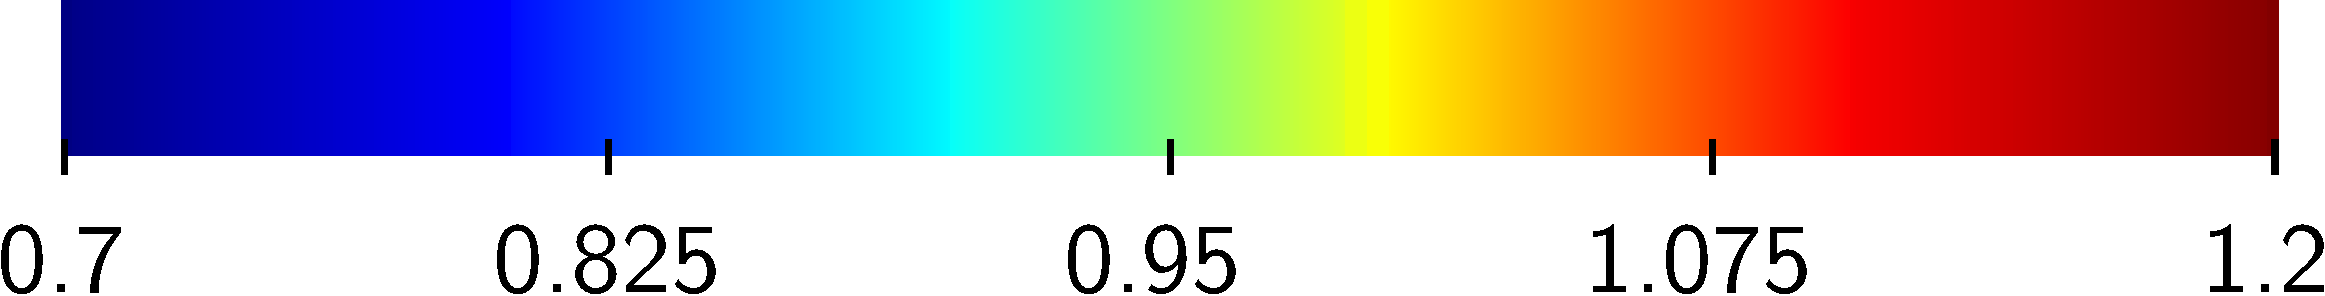
\includegraphics[width=0.22\textwidth]{dream_ls_blade_resp_scale_mean.pdf}} 
   & \multicolumn{2}{c}{
        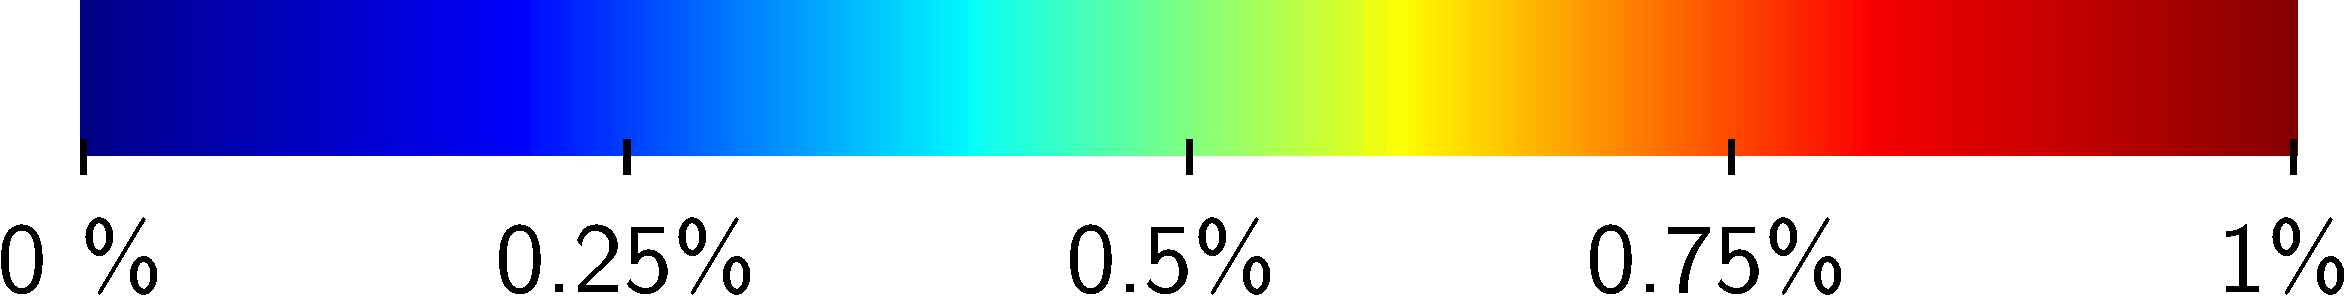
\includegraphics[width=0.22\textwidth]{dream_ls_blade_resp_scale_H01.pdf}} \\
   \midrule
   \rotatebox{90}{\quad\quad\quad steady} 
   & 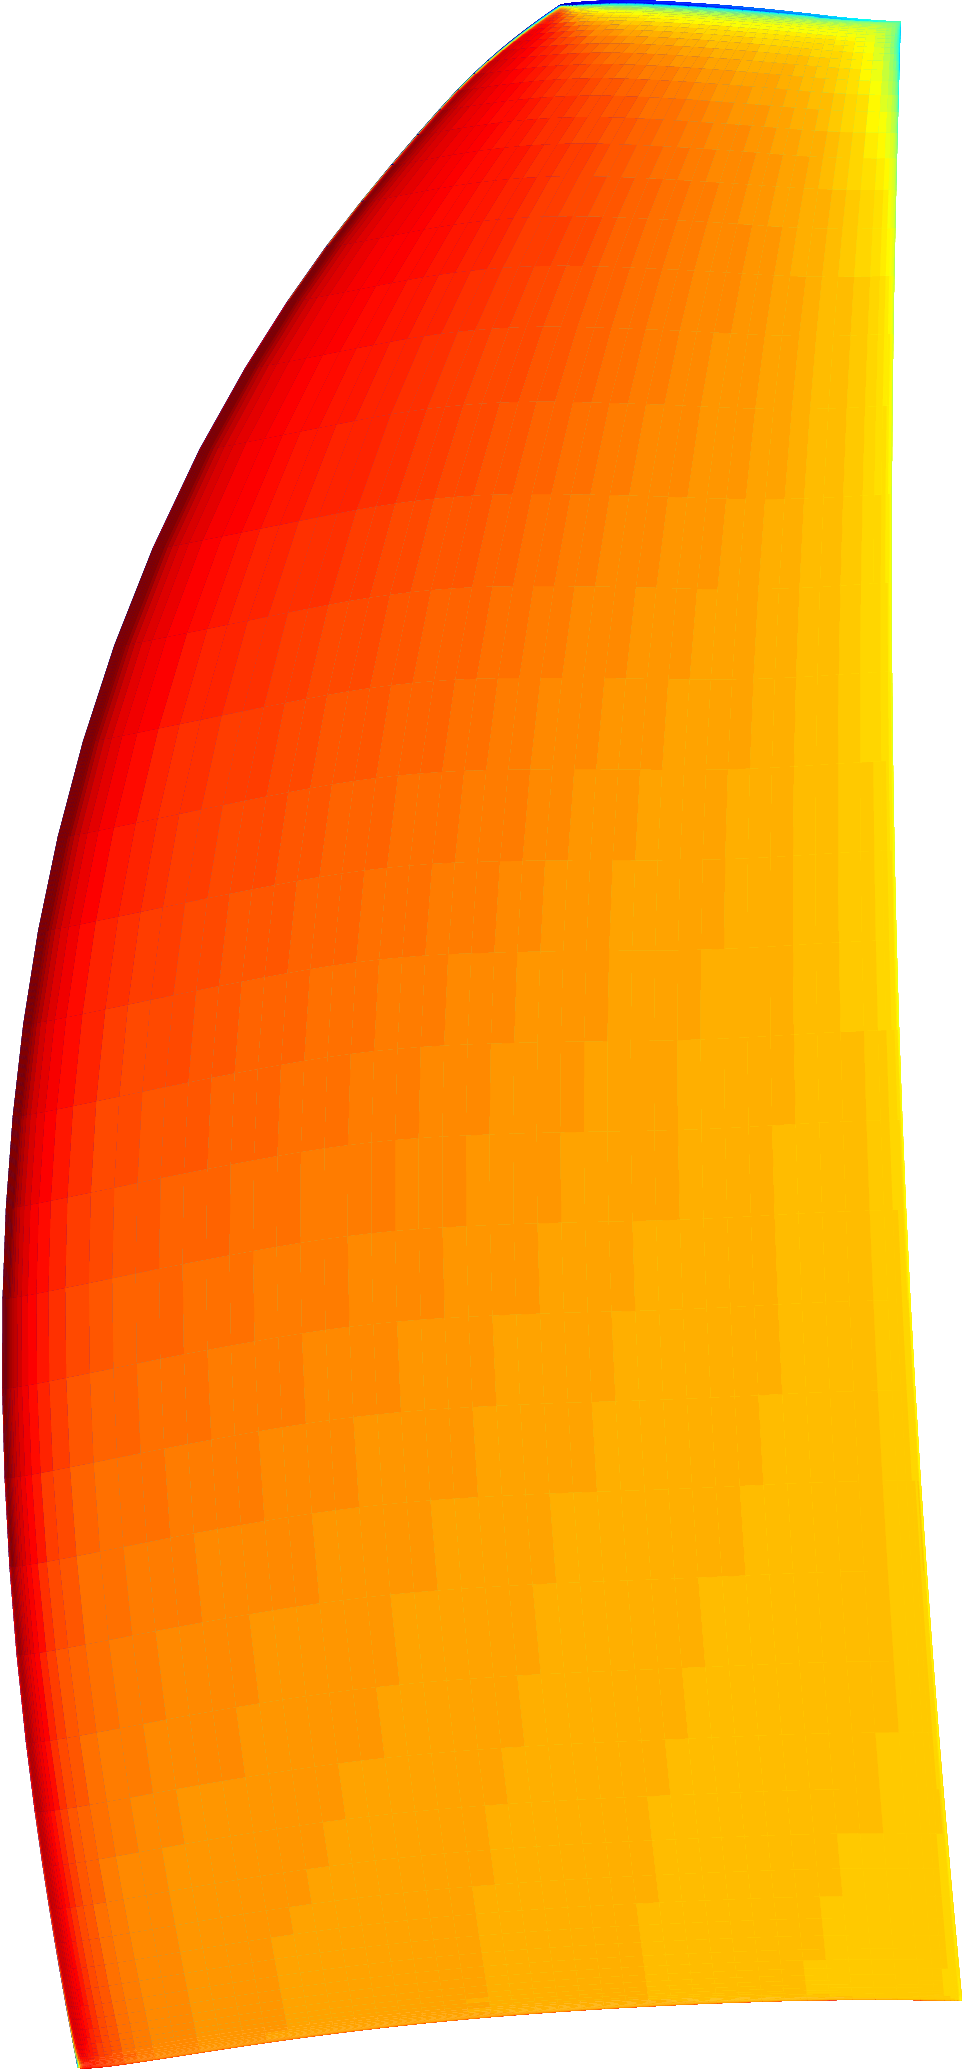
\includegraphics[width=0.10\textwidth]{DREAM_LS_RANS_roe2_sa_blade_response_rear_PS.png}
   & 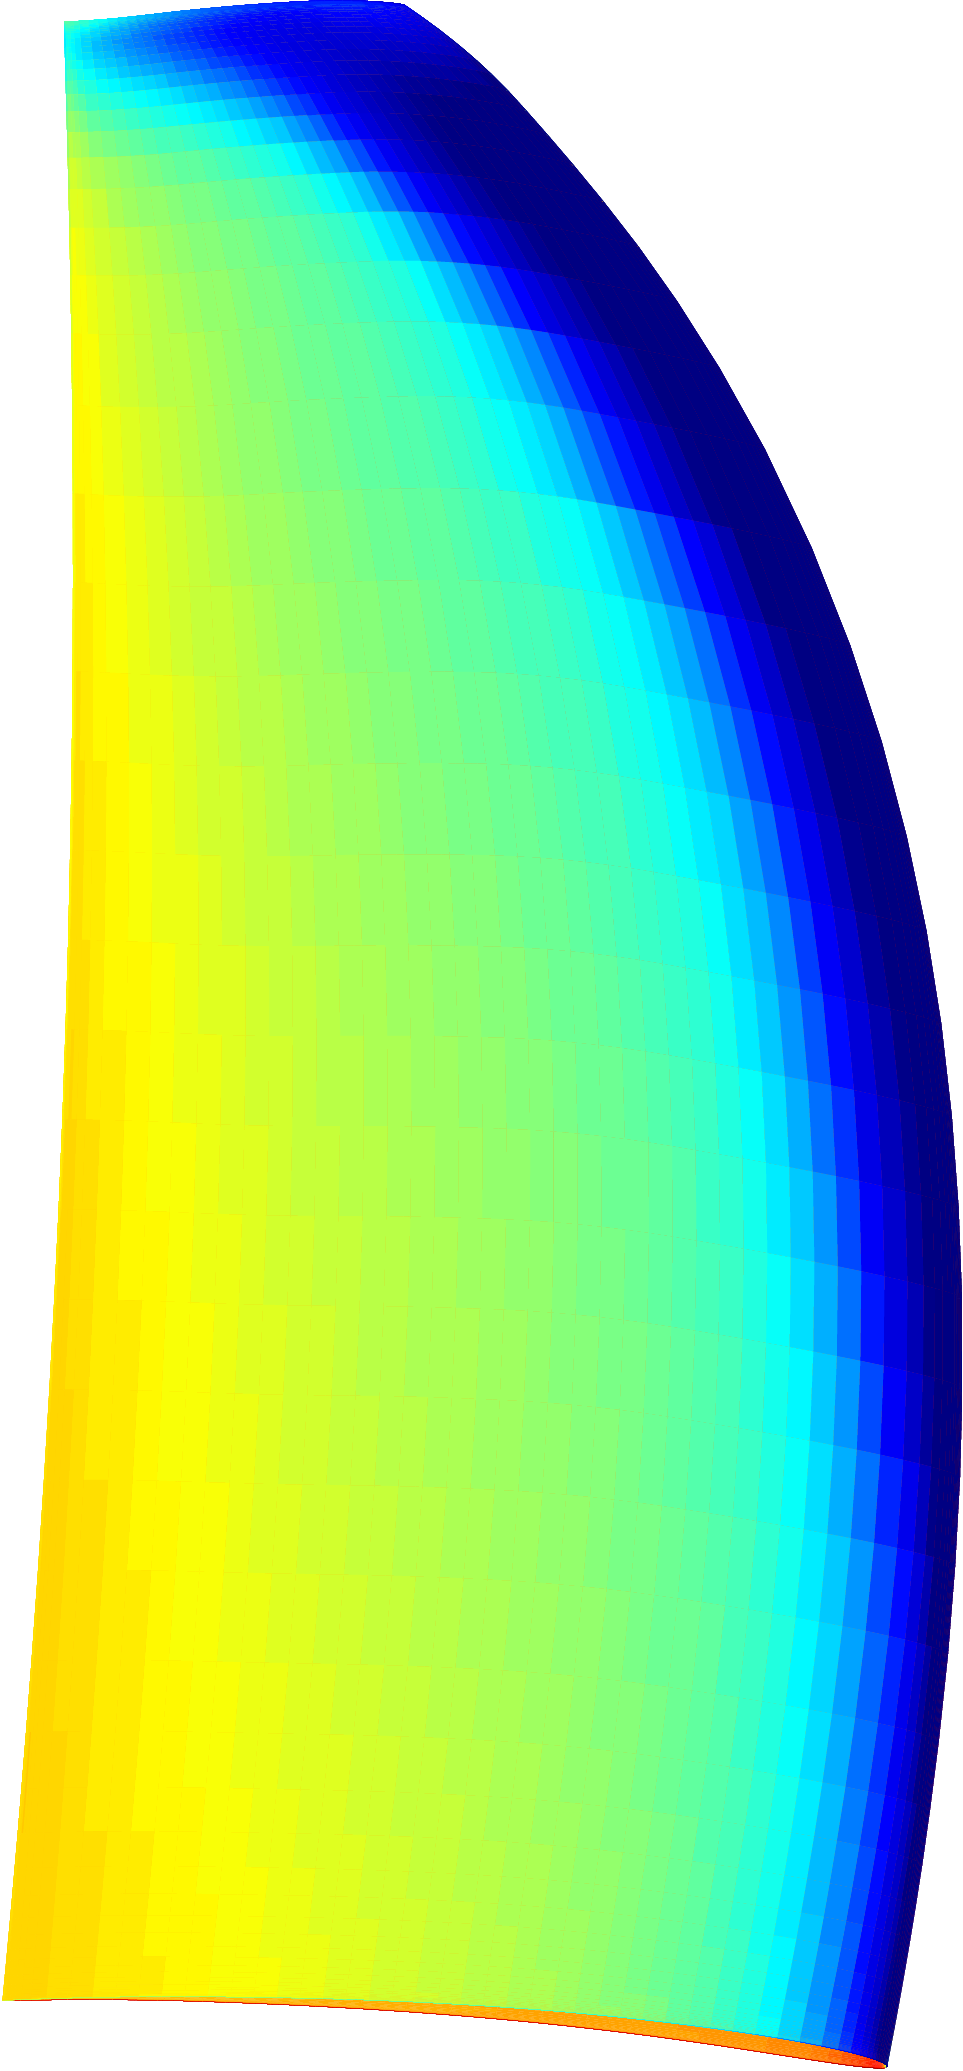
\includegraphics[width=0.10\textwidth]{DREAM_LS_RANS_roe2_sa_blade_response_rear_SS.png}
   &   &\\
   \rotatebox{90}{\quad\quad HB $N=1$} 
   & 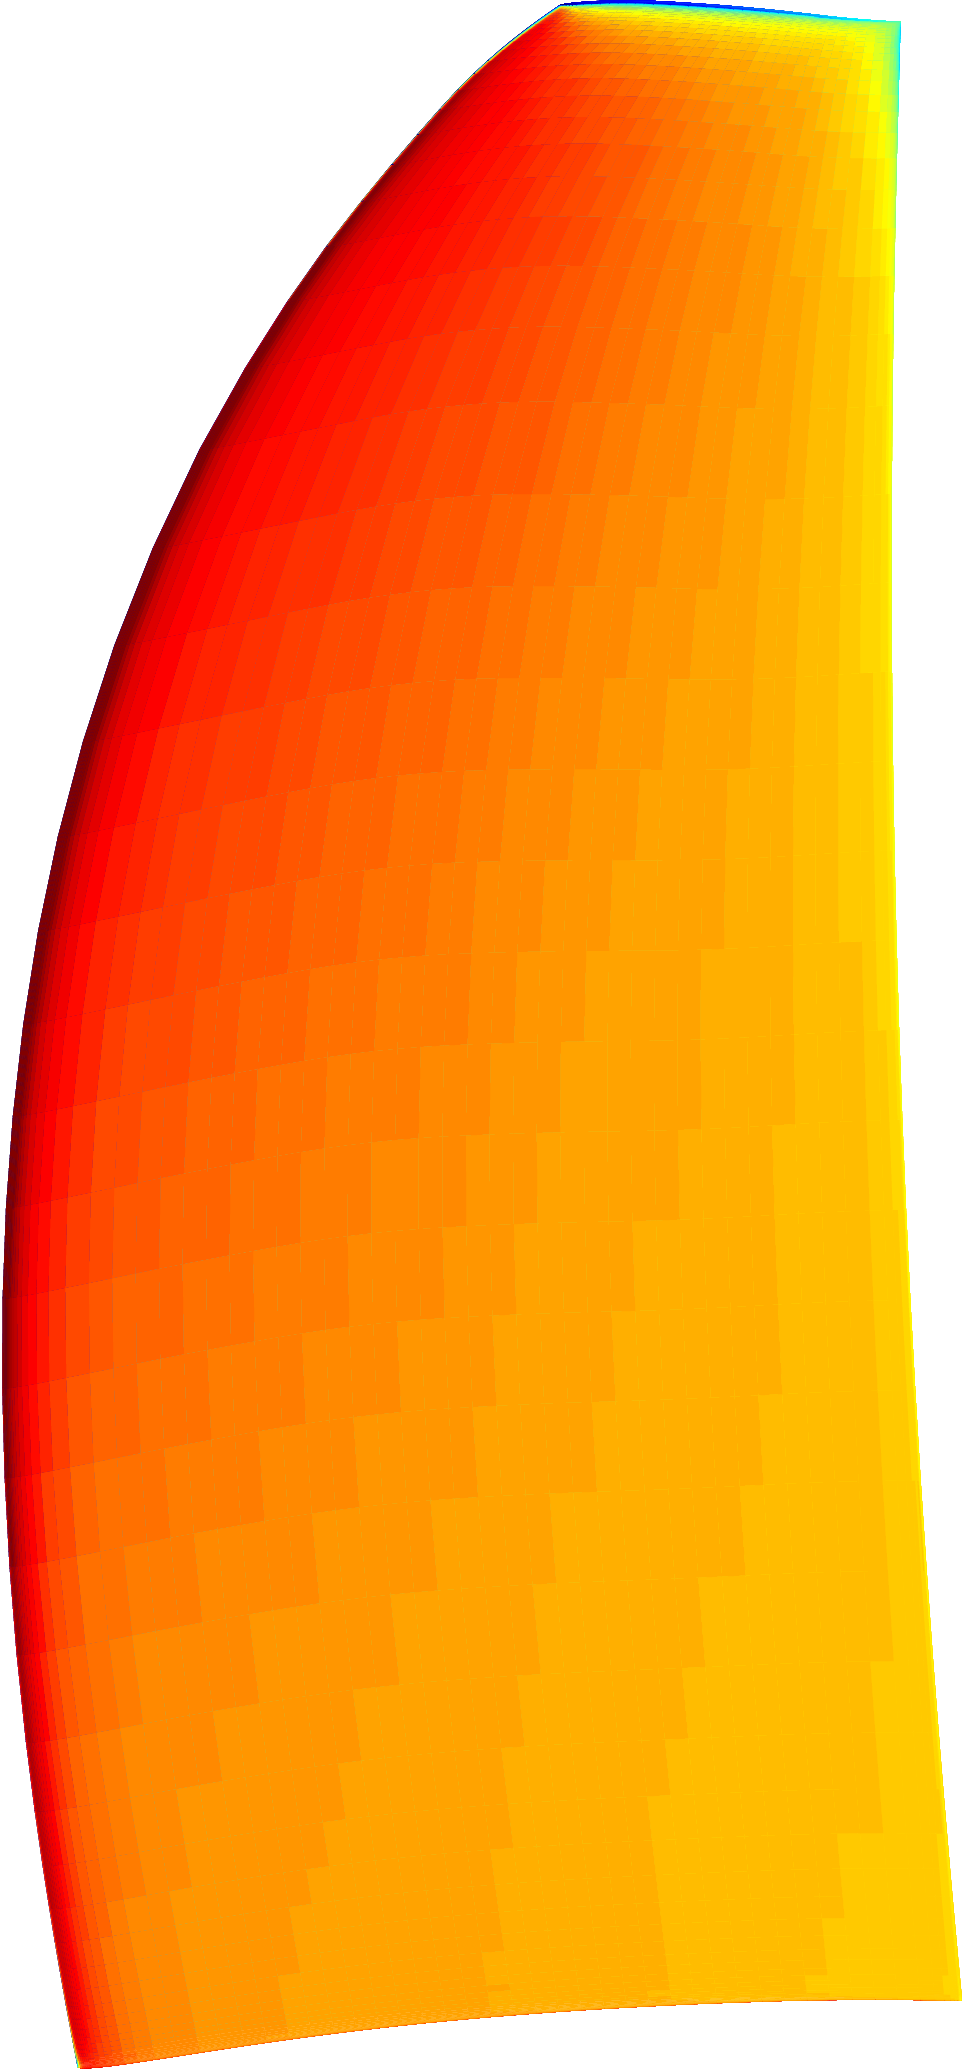
\includegraphics[width=0.10\textwidth]{DREAM_LS_TSM_N1_roe2_sa_blade_response_rear_mean_PS.png}
   & 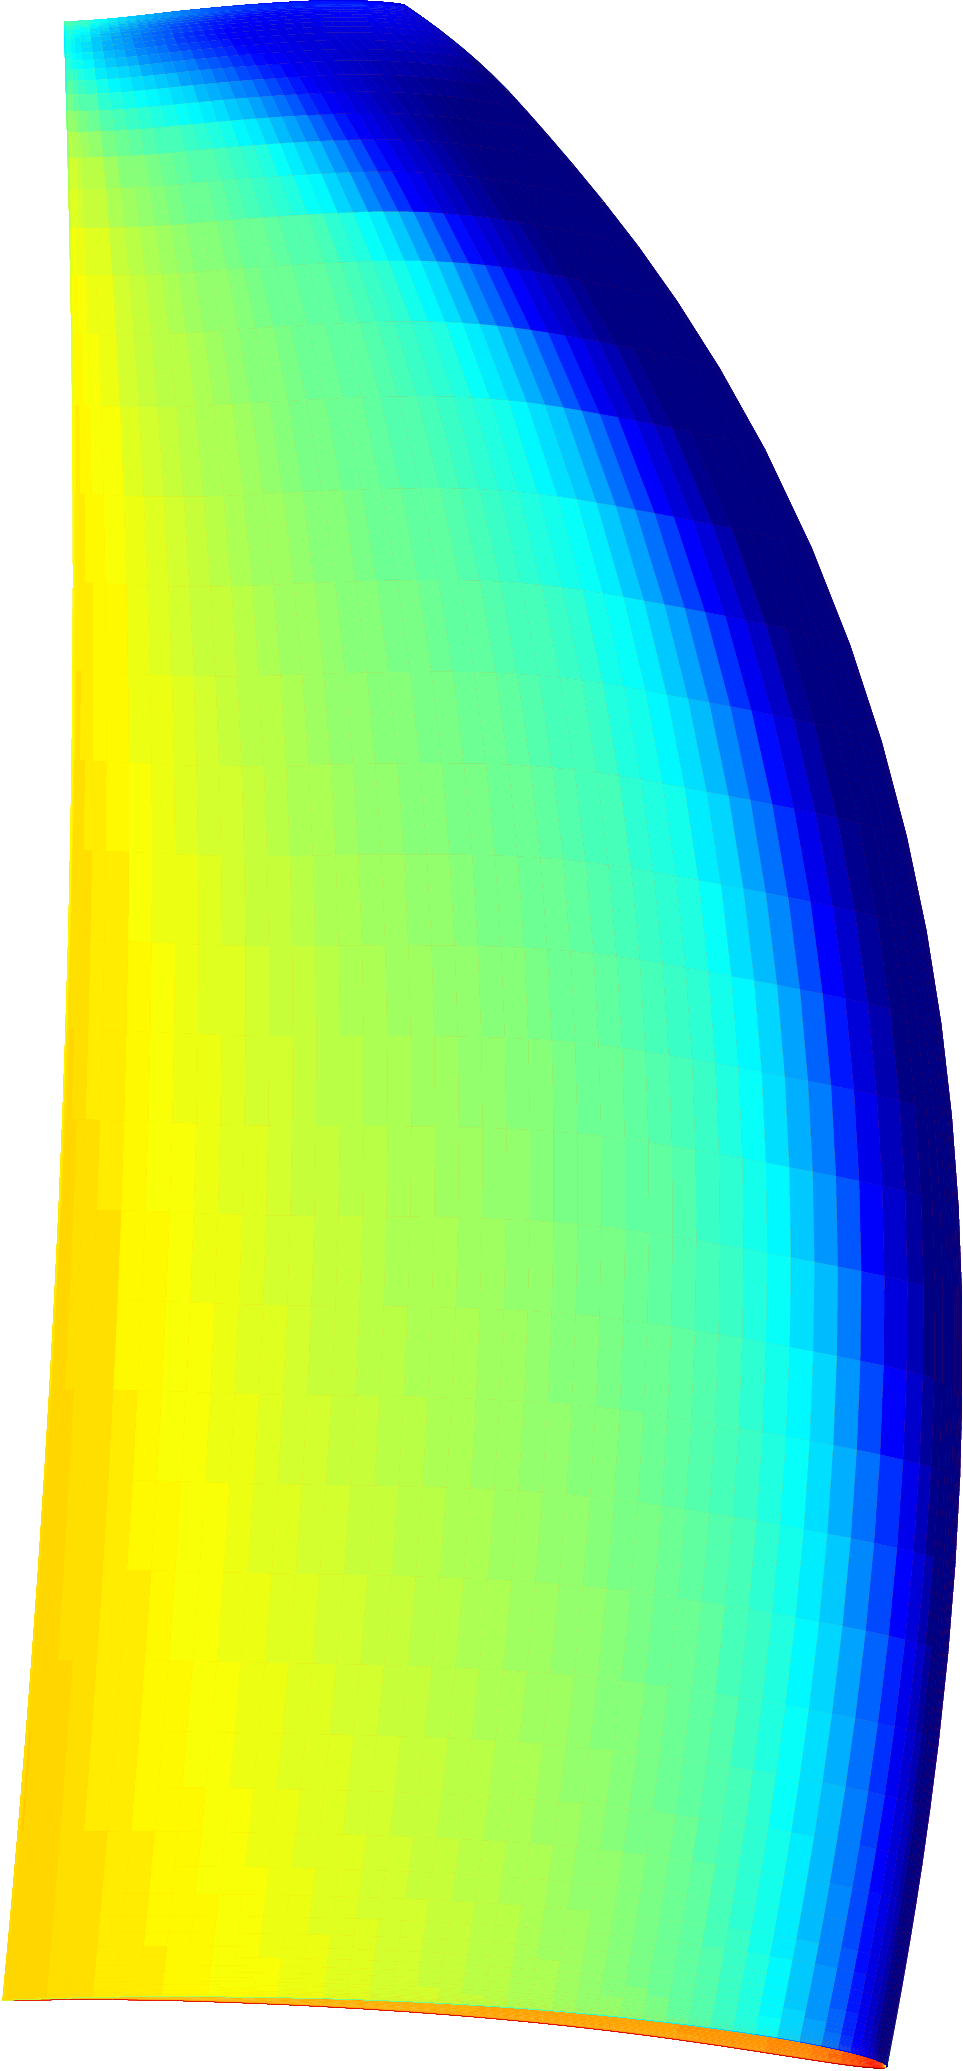
\includegraphics[width=0.10\textwidth]{DREAM_LS_TSM_N1_roe2_sa_blade_response_rear_mean_SS.png}
   & 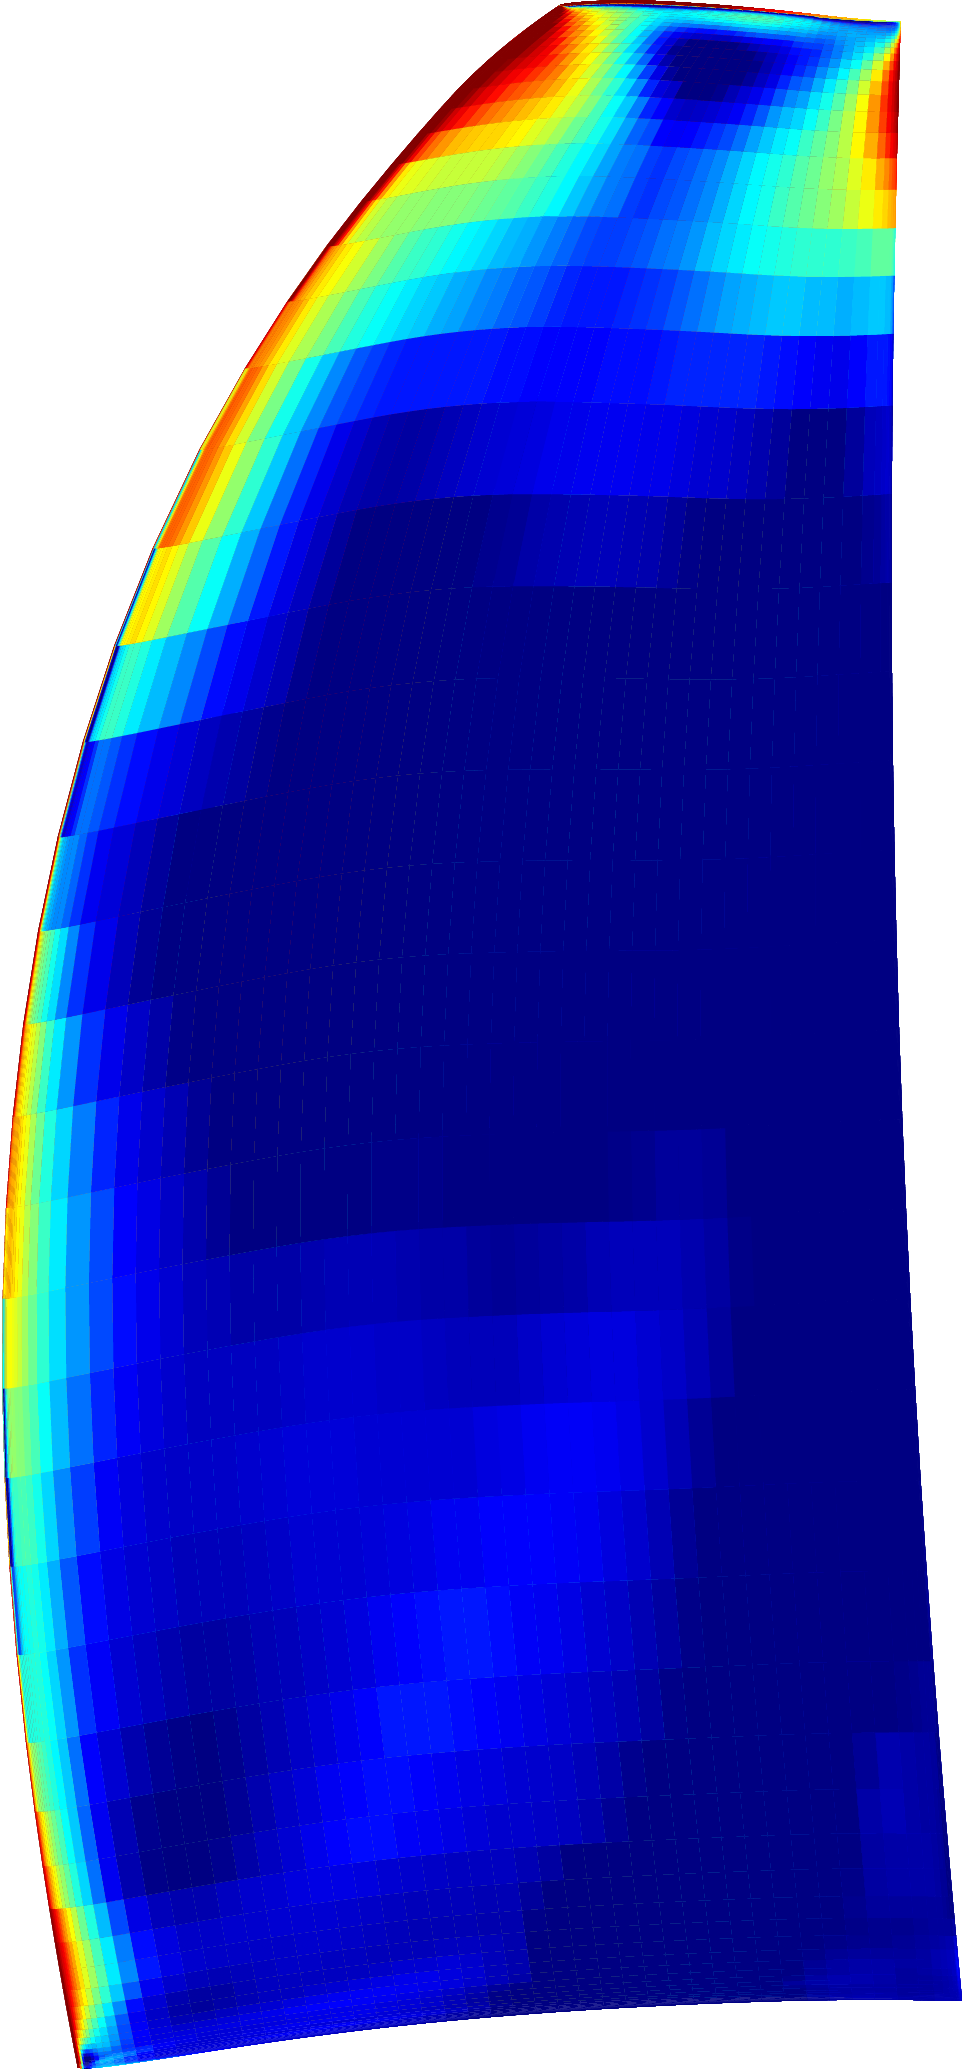
\includegraphics[width=0.10\textwidth]{DREAM_LS_TSM_N1_roe2_sa_blade_response_rear_H01_PS.png}
   & 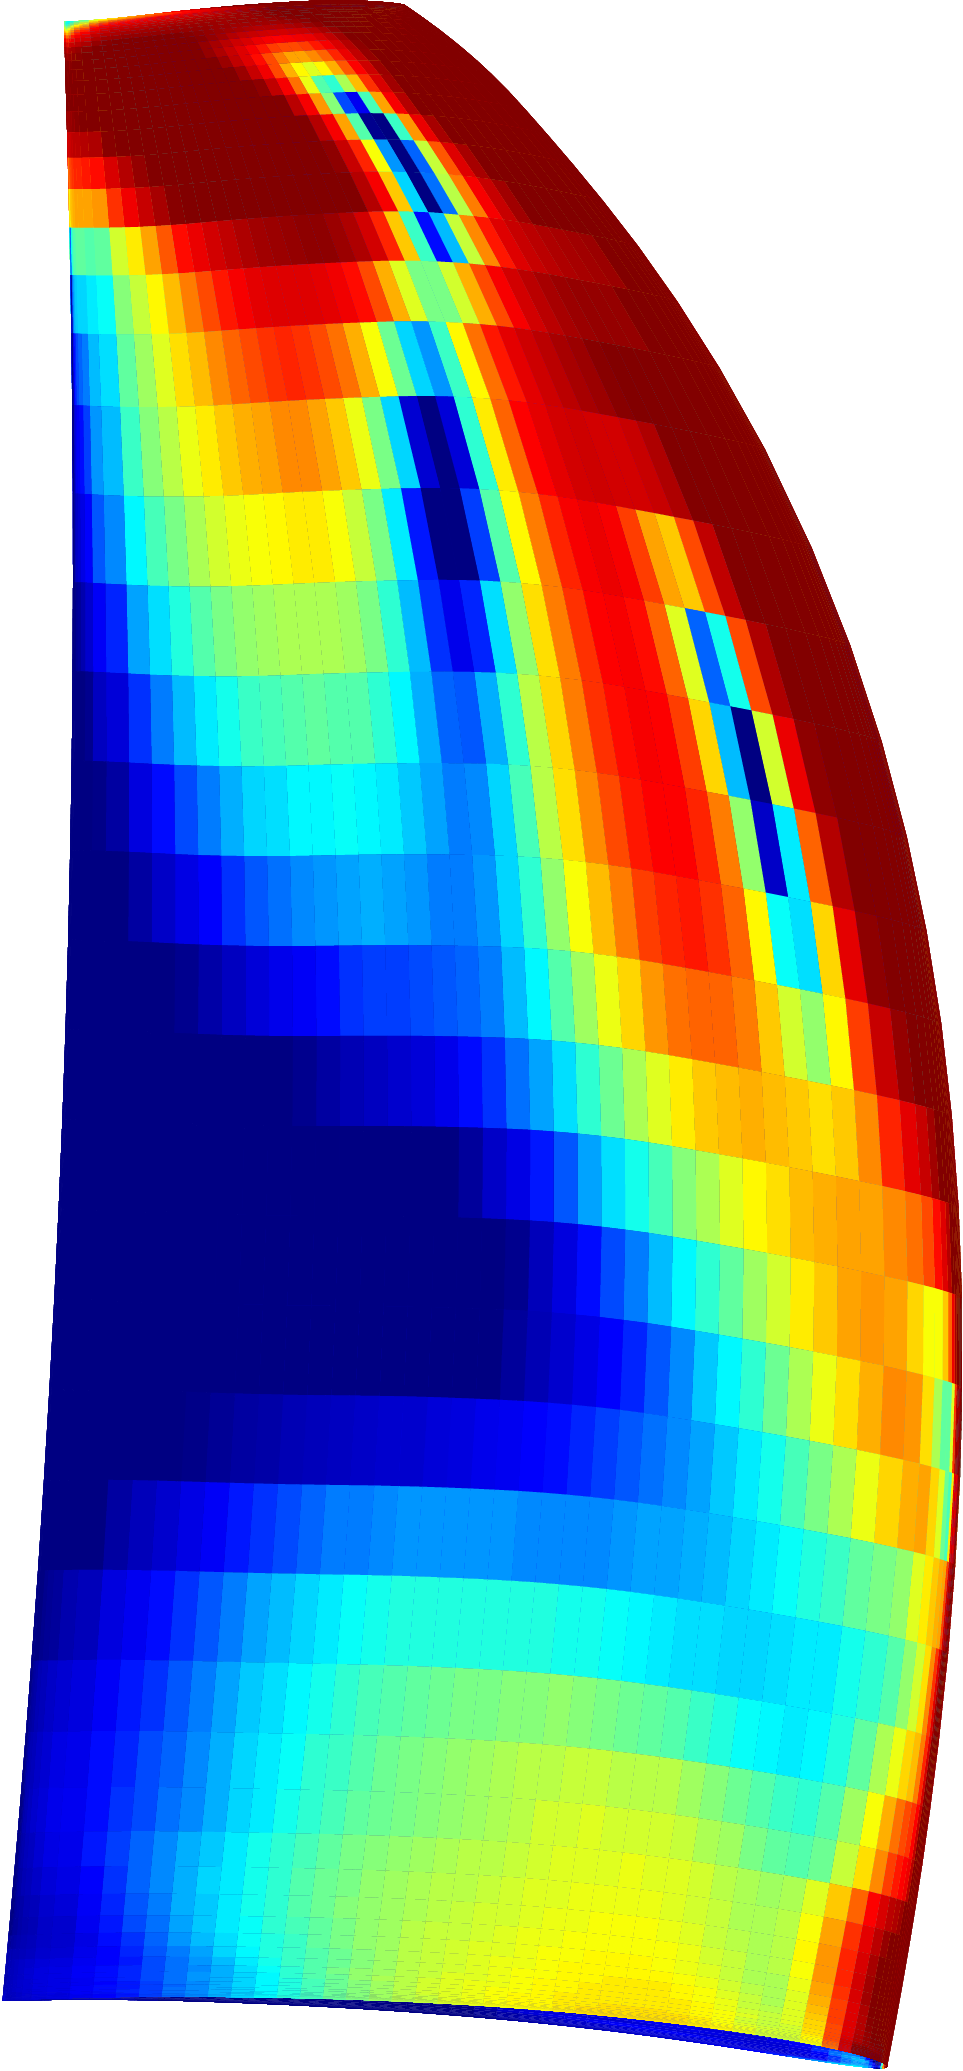
\includegraphics[width=0.10\textwidth]{DREAM_LS_TSM_N1_roe2_sa_blade_response_rear_H01_SS.png} \\
   \rotatebox{90}{\quad\quad HB $N=2$} 
   & 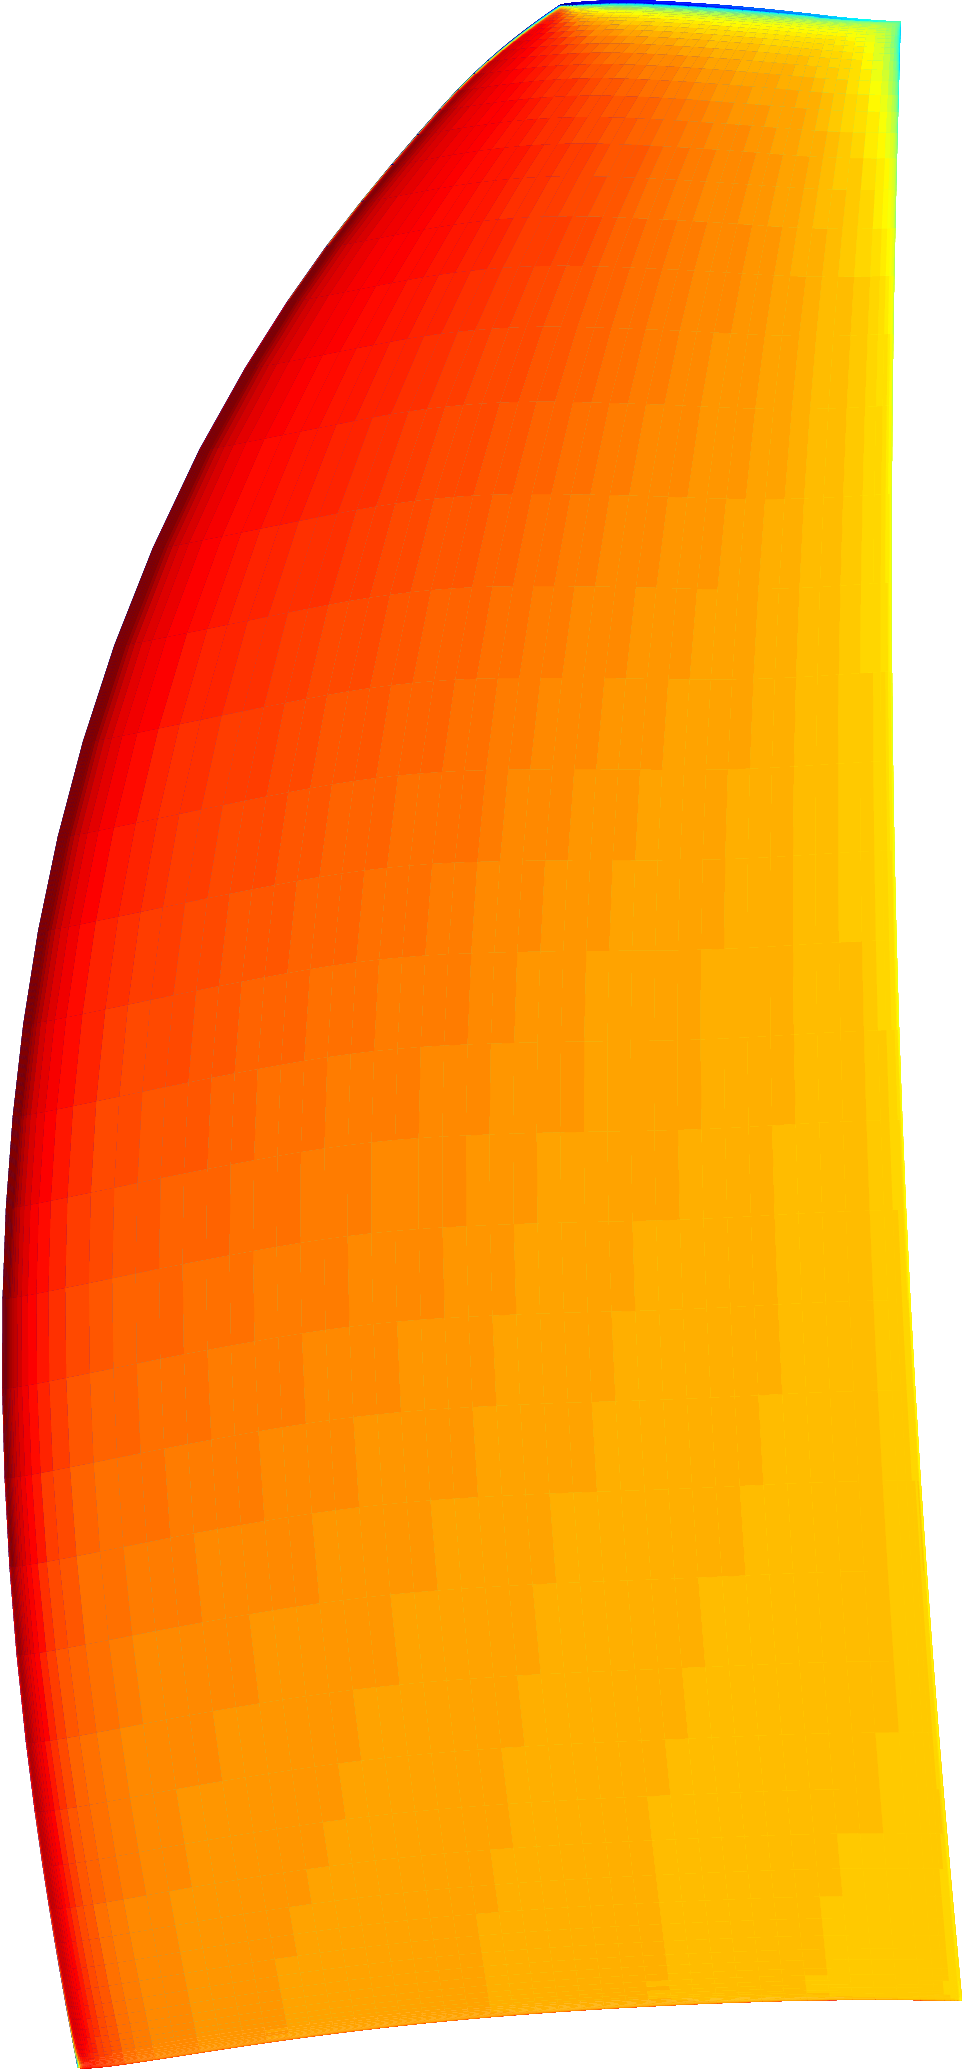
\includegraphics[width=0.10\textwidth]{DREAM_LS_TSM_N2_roe2_sa_blade_response_rear_mean_PS.png}
   & 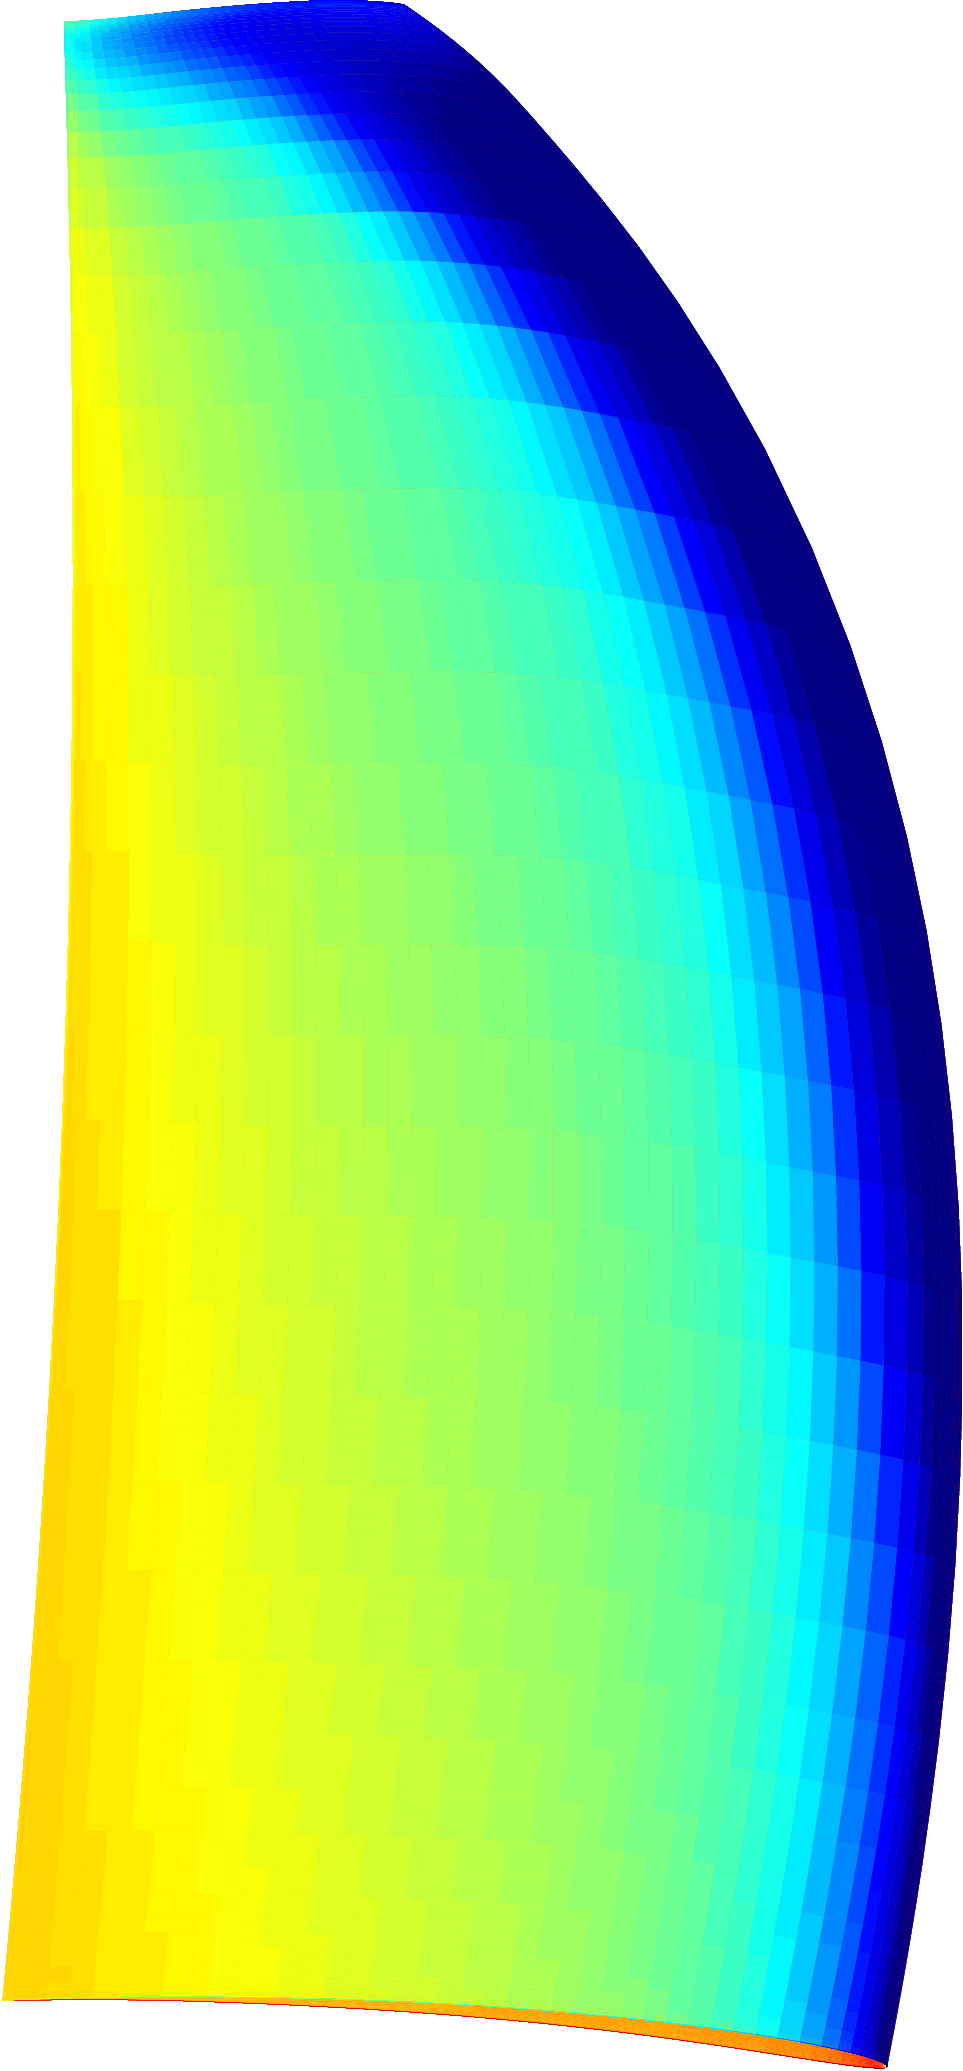
\includegraphics[width=0.10\textwidth]{DREAM_LS_TSM_N2_roe2_sa_blade_response_rear_mean_SS.png}
   & 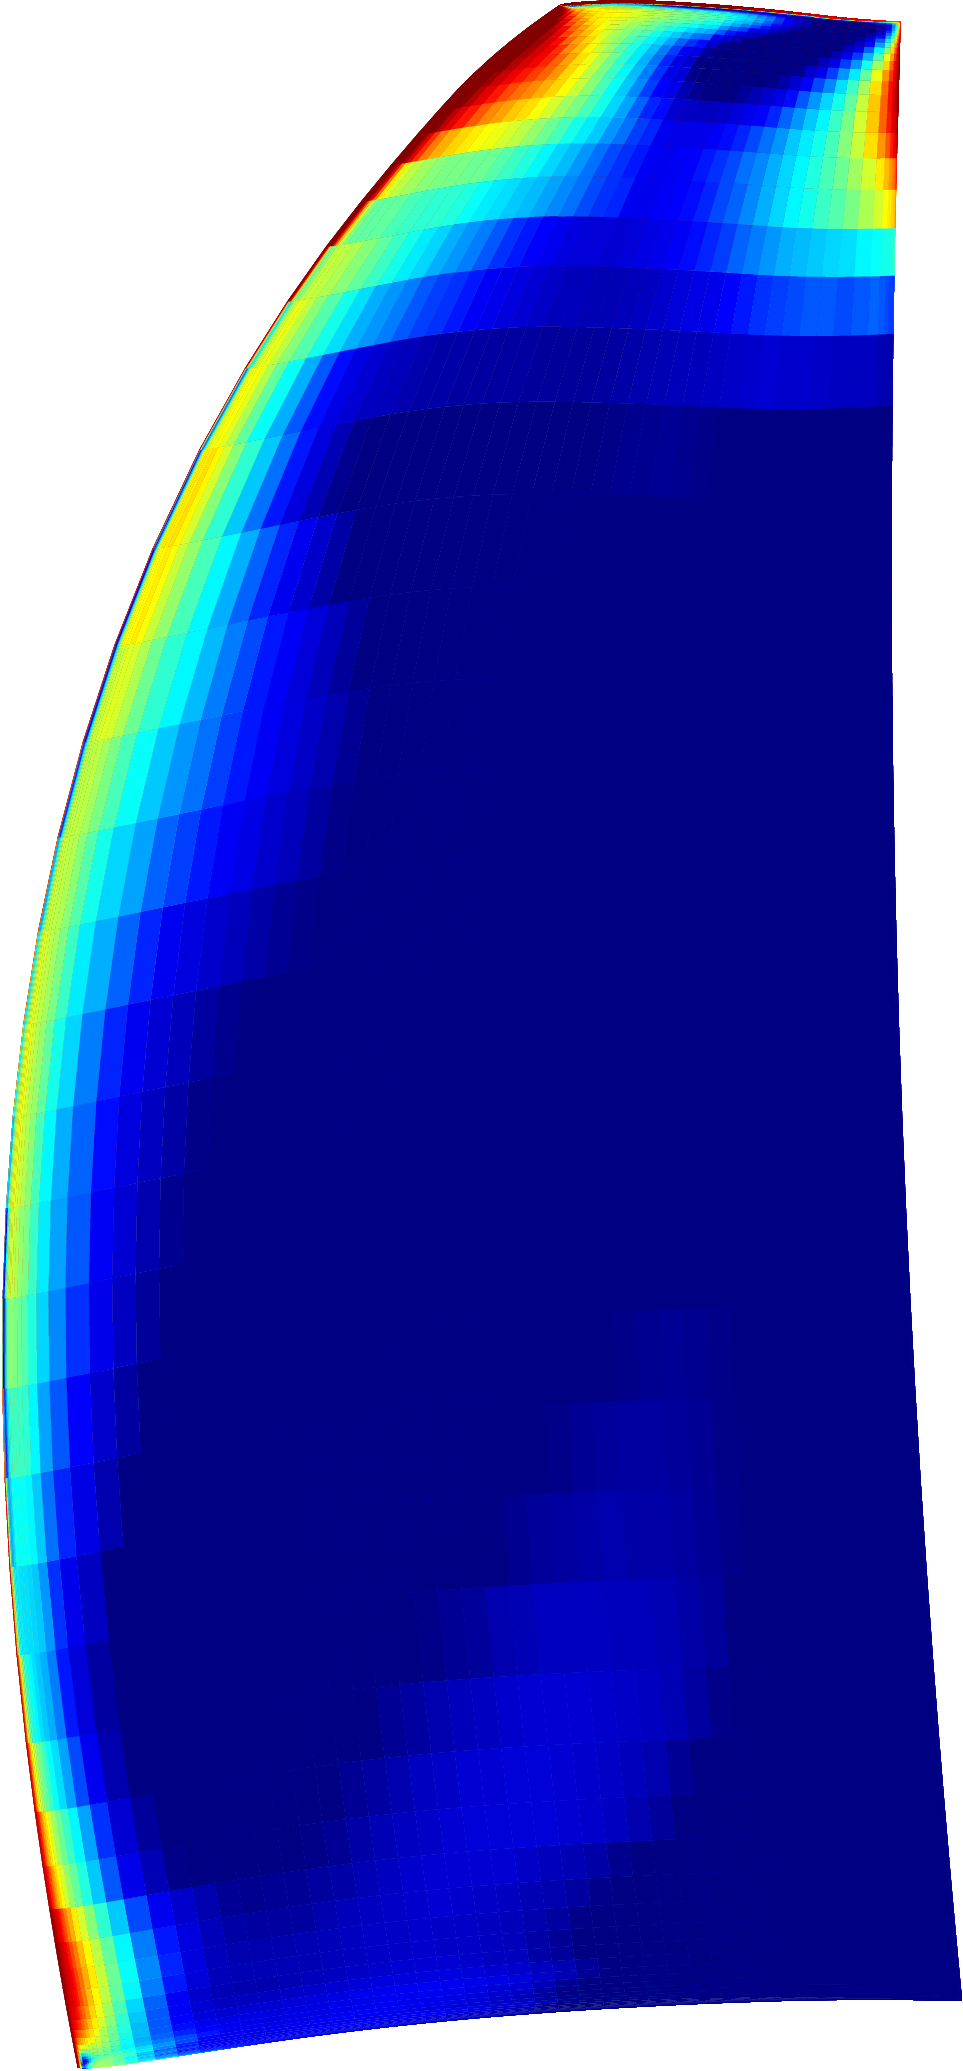
\includegraphics[width=0.10\textwidth]{DREAM_LS_TSM_N2_roe2_sa_blade_response_rear_H01_PS.png}
   & 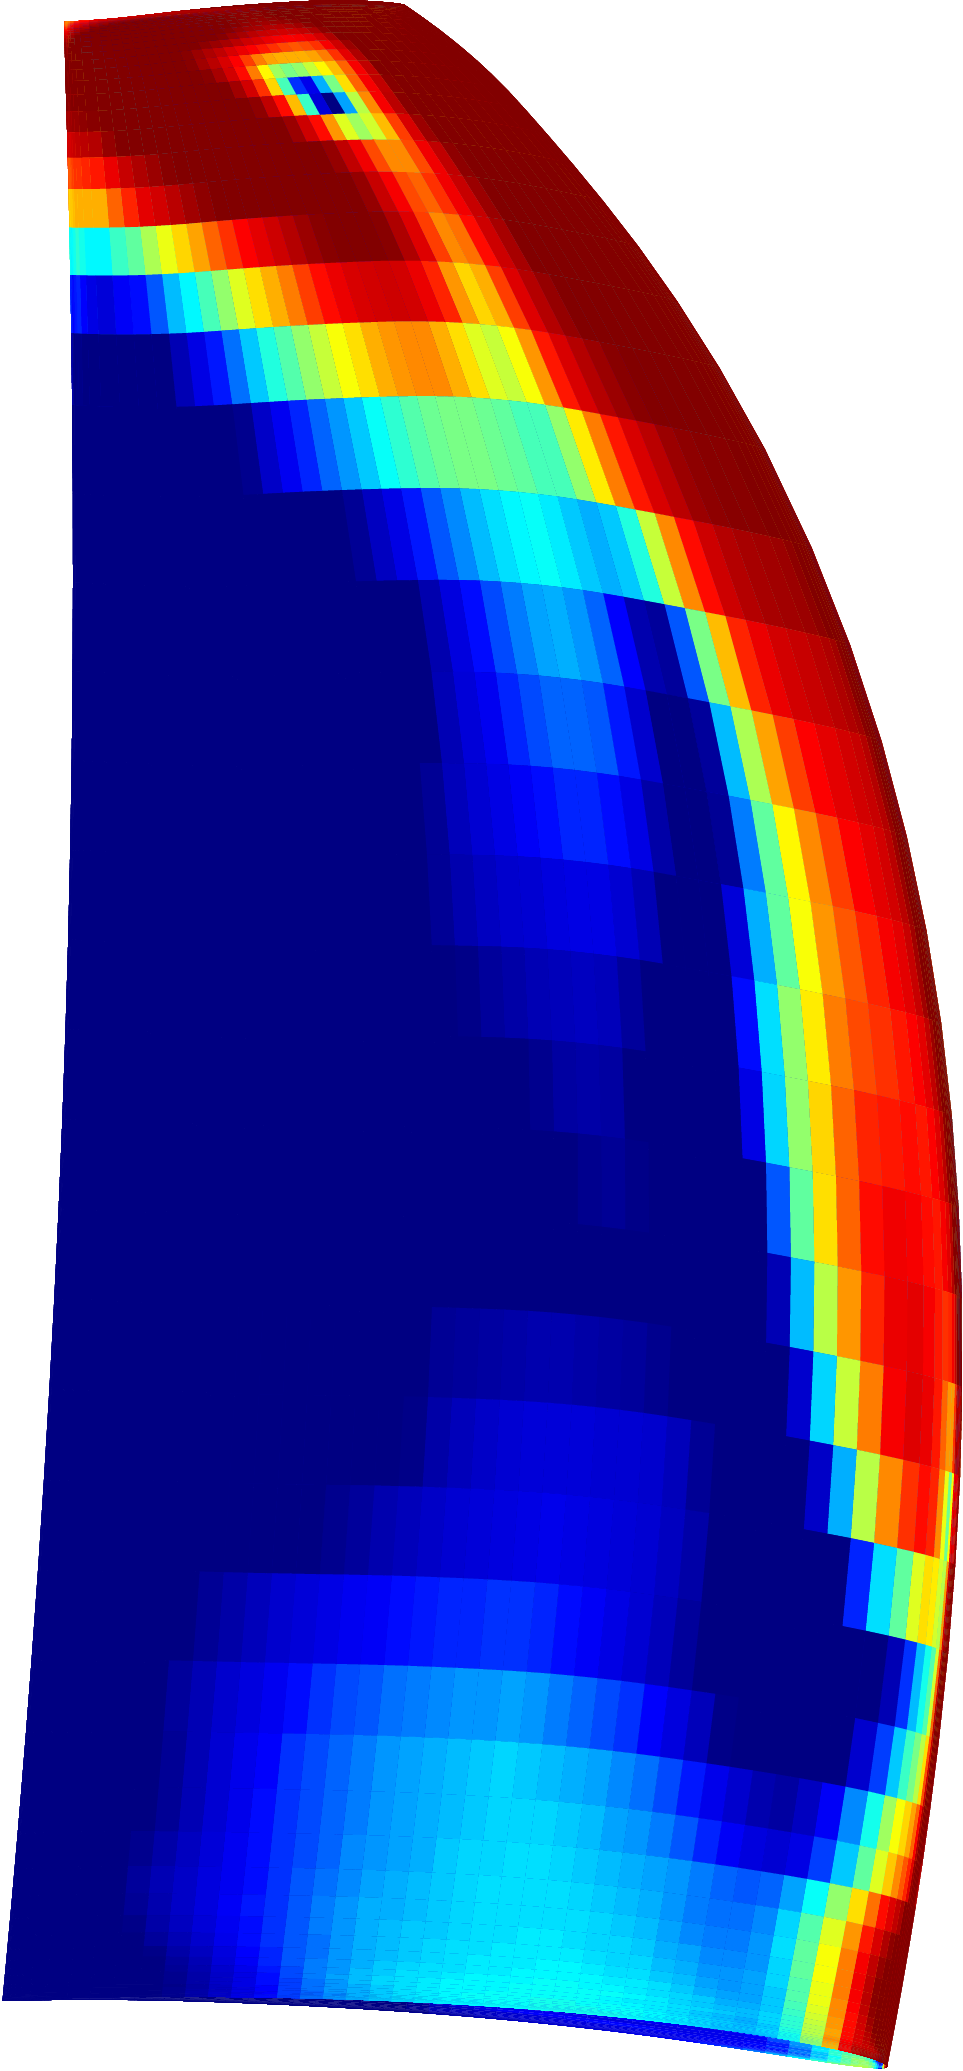
\includegraphics[width=0.10\textwidth]{DREAM_LS_TSM_N2_roe2_sa_blade_response_rear_H01_SS.png} \\
   \rotatebox{90}{\quad\quad HB $N=3$} 
   & 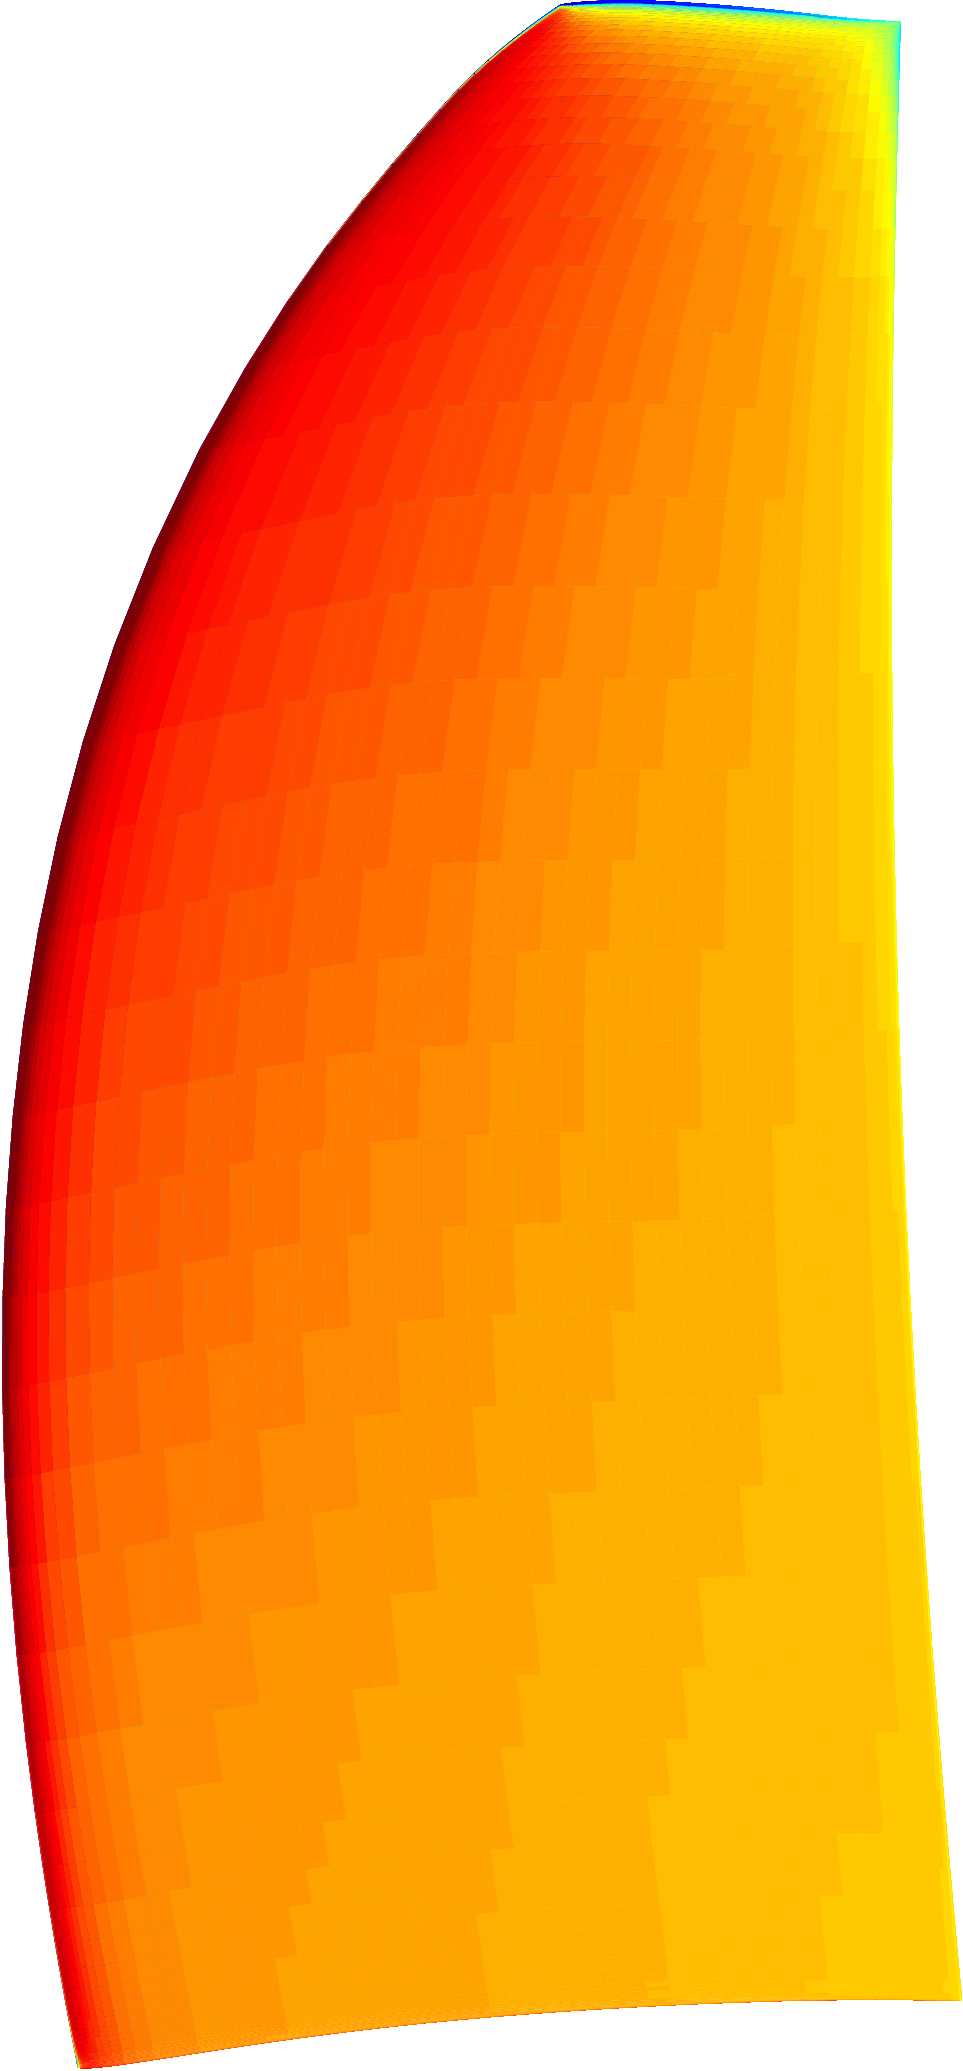
\includegraphics[width=0.10\textwidth]{DREAM_LS_TSM_N3_roe2_sa_blade_response_rear_mean_PS.png}
   & 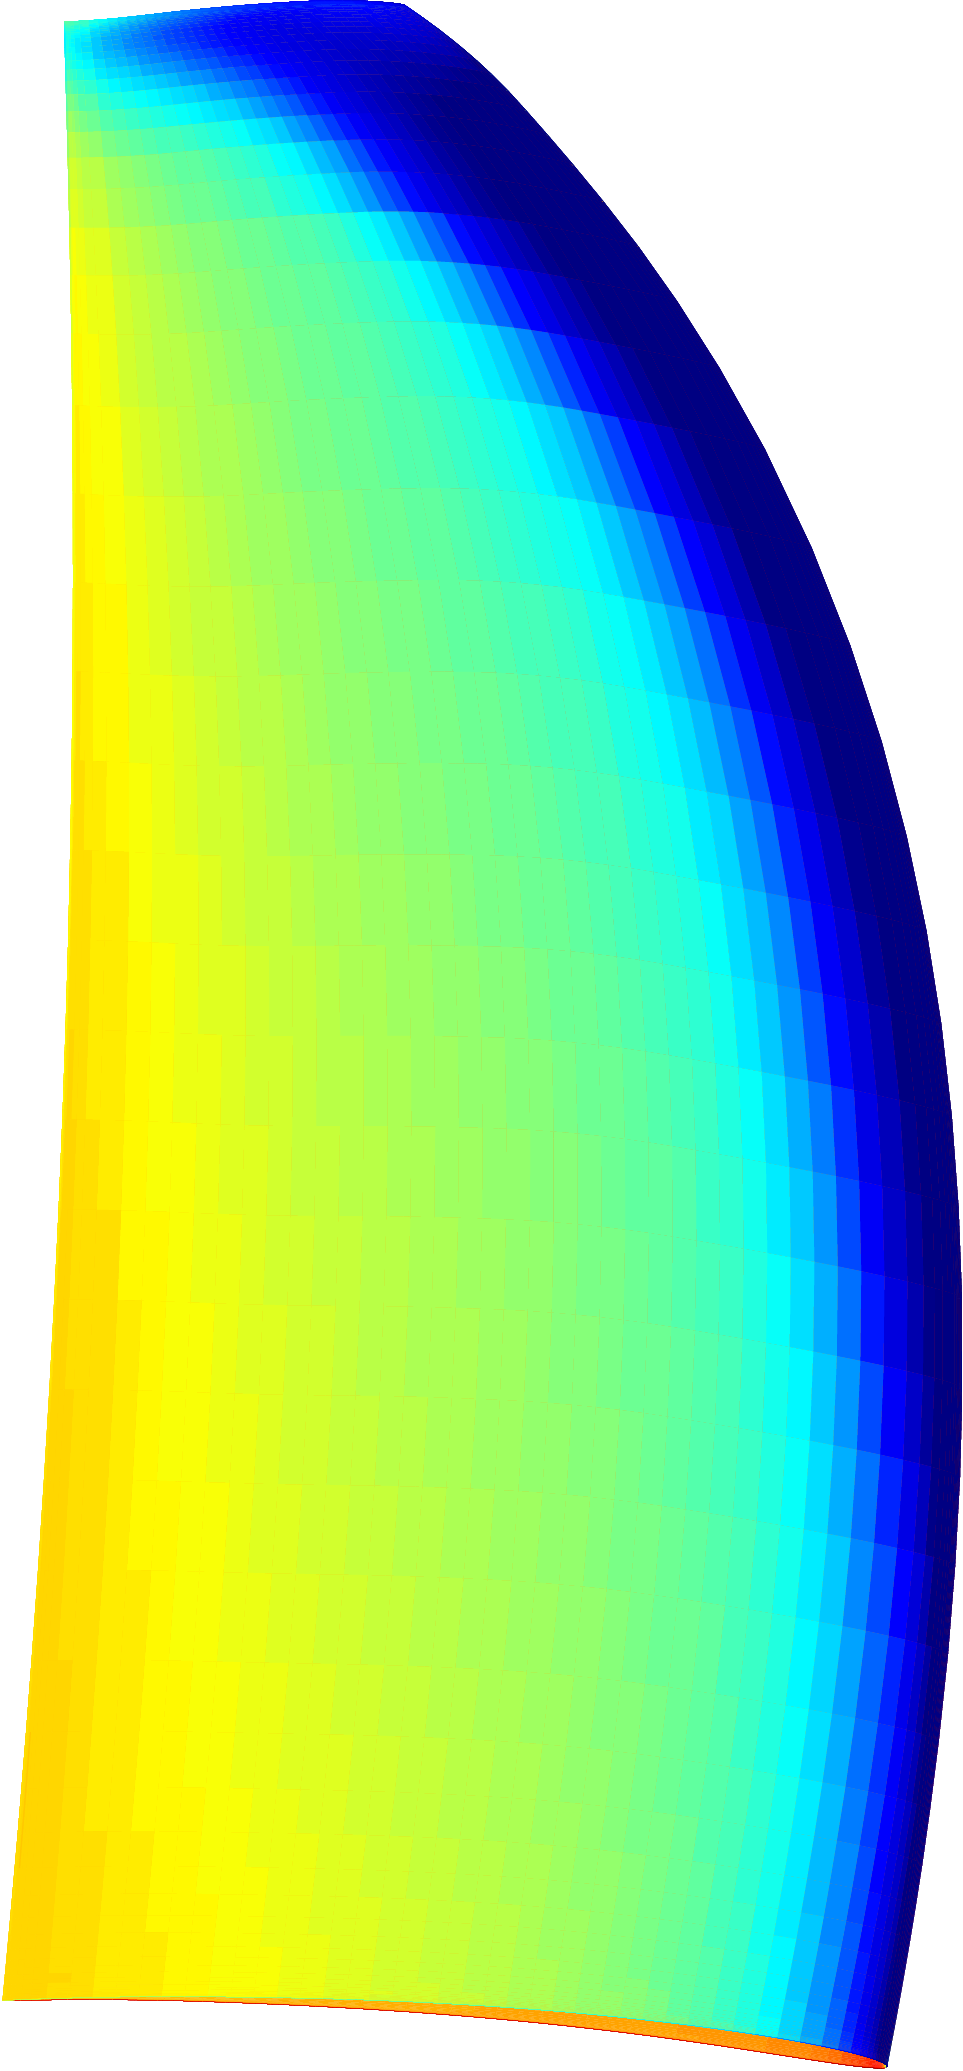
\includegraphics[width=0.10\textwidth]{DREAM_LS_TSM_N3_roe2_sa_blade_response_rear_mean_SS.png}
   & 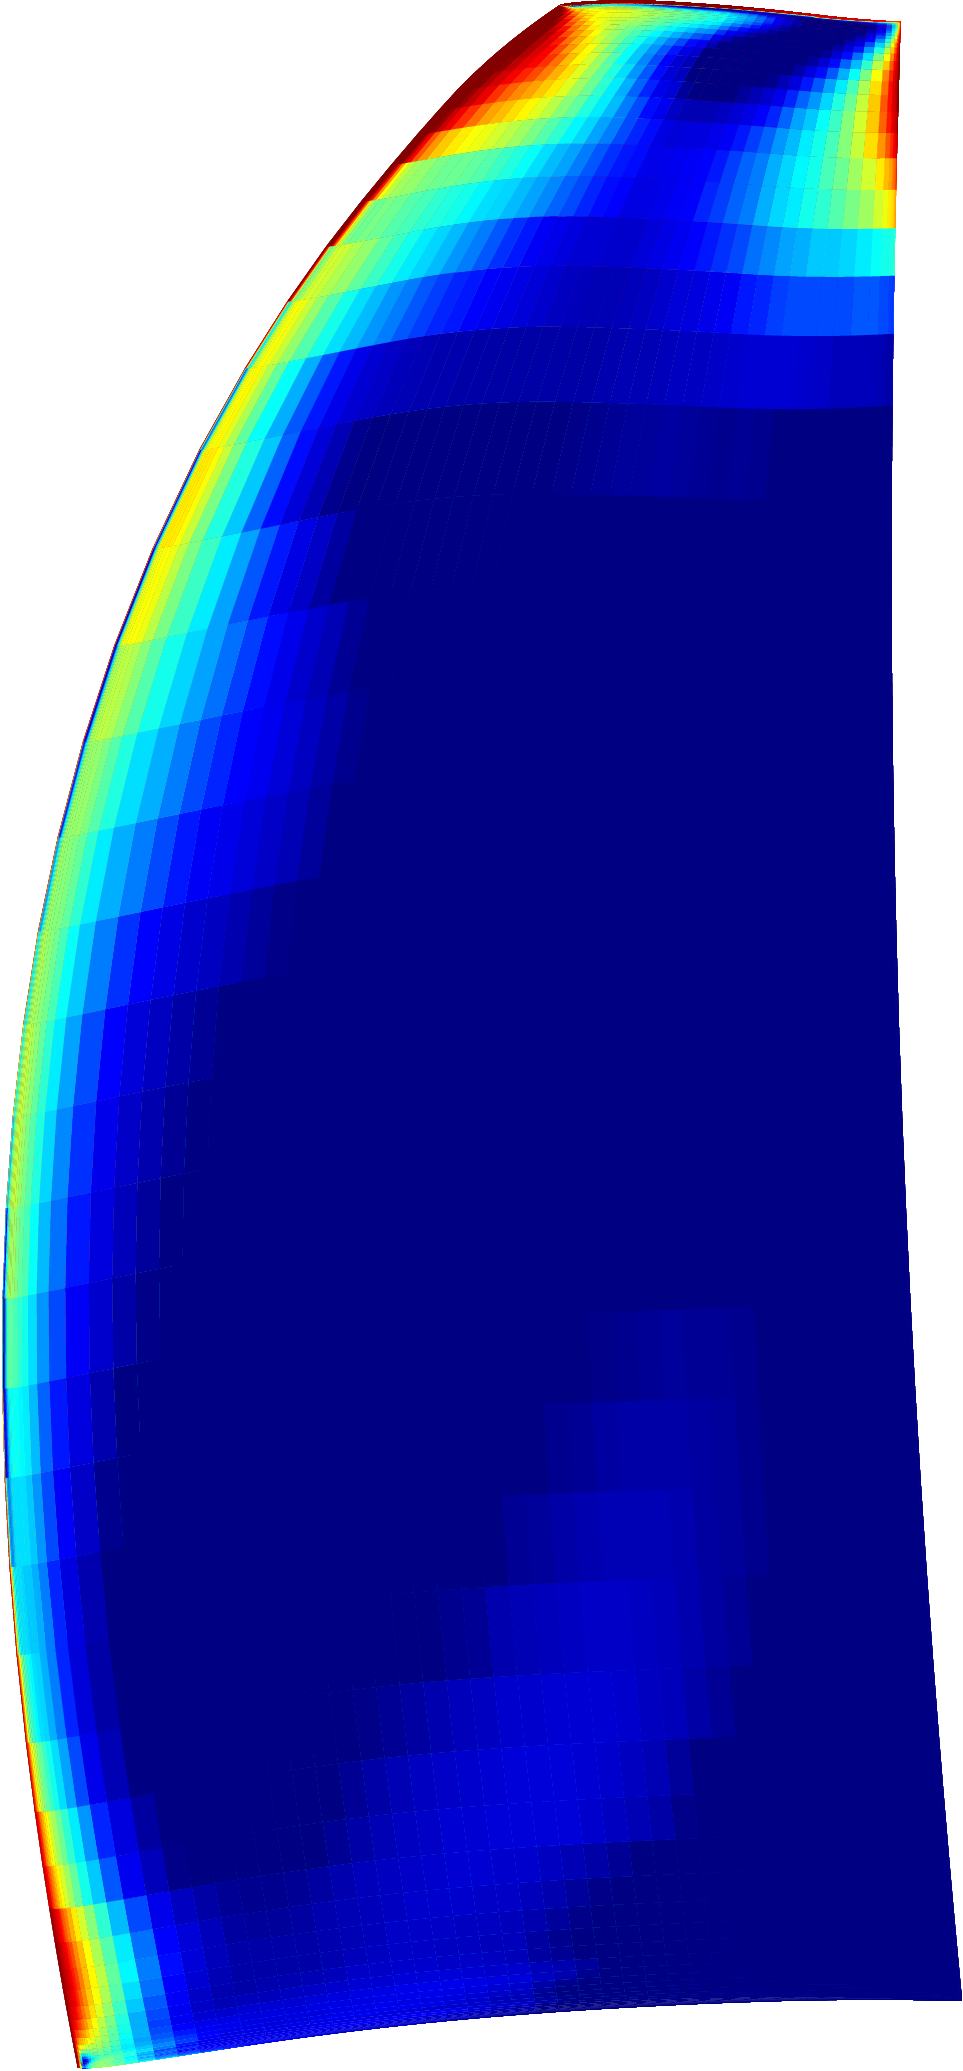
\includegraphics[width=0.10\textwidth]{DREAM_LS_TSM_N3_roe2_sa_blade_response_rear_H01_PS.png}
   & 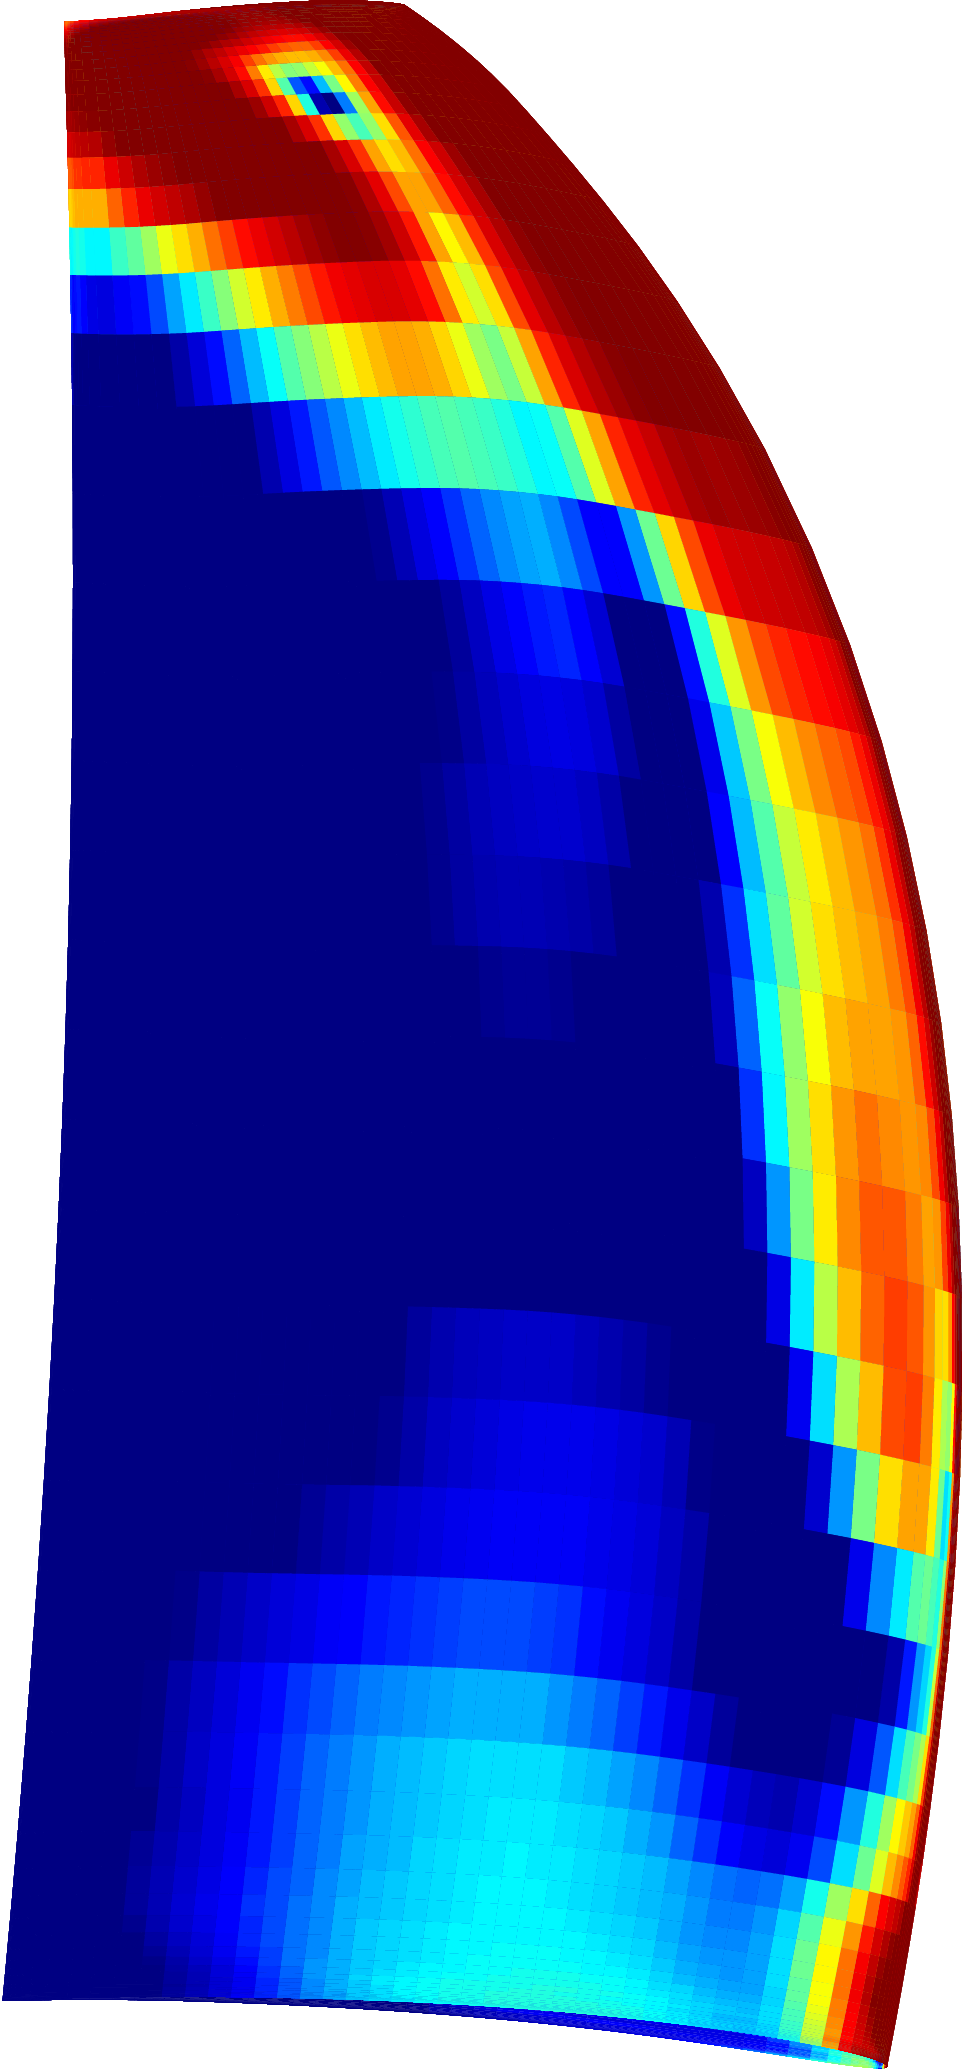
\includegraphics[width=0.10\textwidth]{DREAM_LS_TSM_N3_roe2_sa_blade_response_rear_H01_SS.png} \\
   \rotatebox{90}{\quad\quad HB $N=4$} 
   & 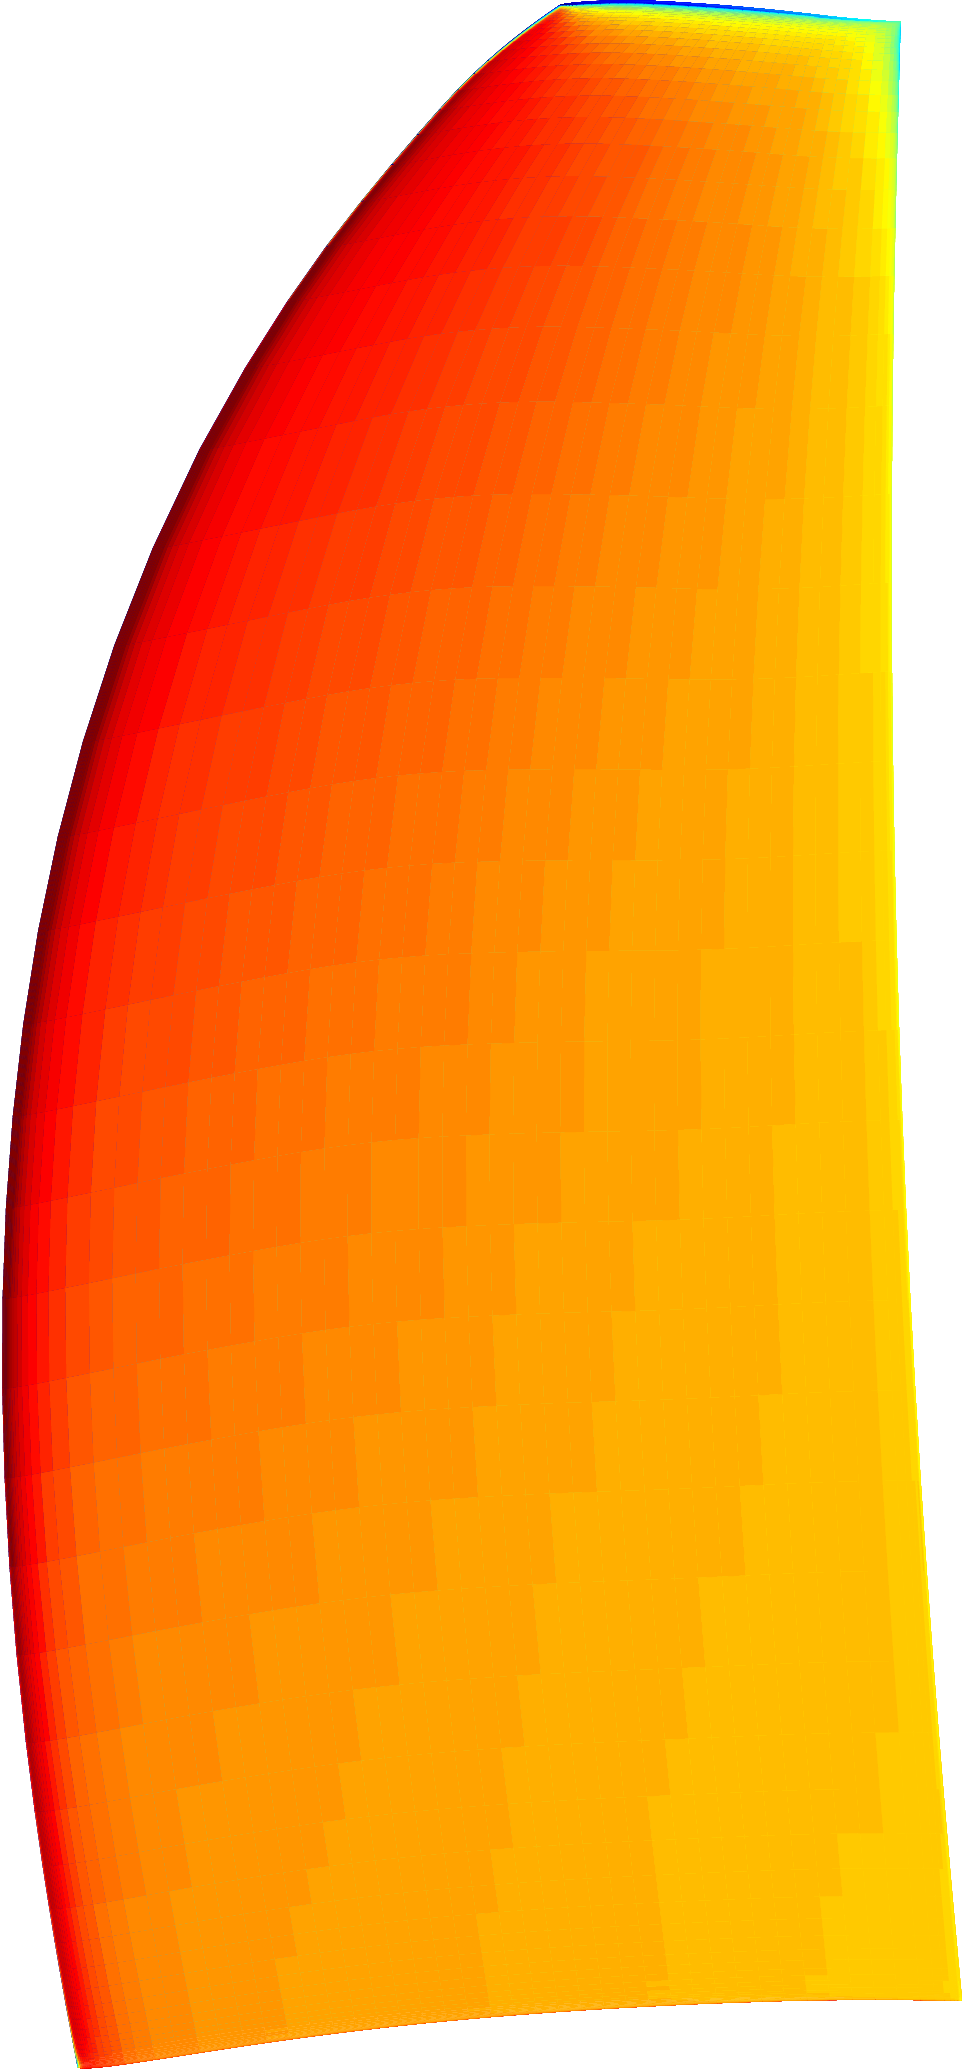
\includegraphics[width=0.10\textwidth]{DREAM_LS_TSM_N4_roe2_sa_blade_response_rear_mean_PS.png}
   & 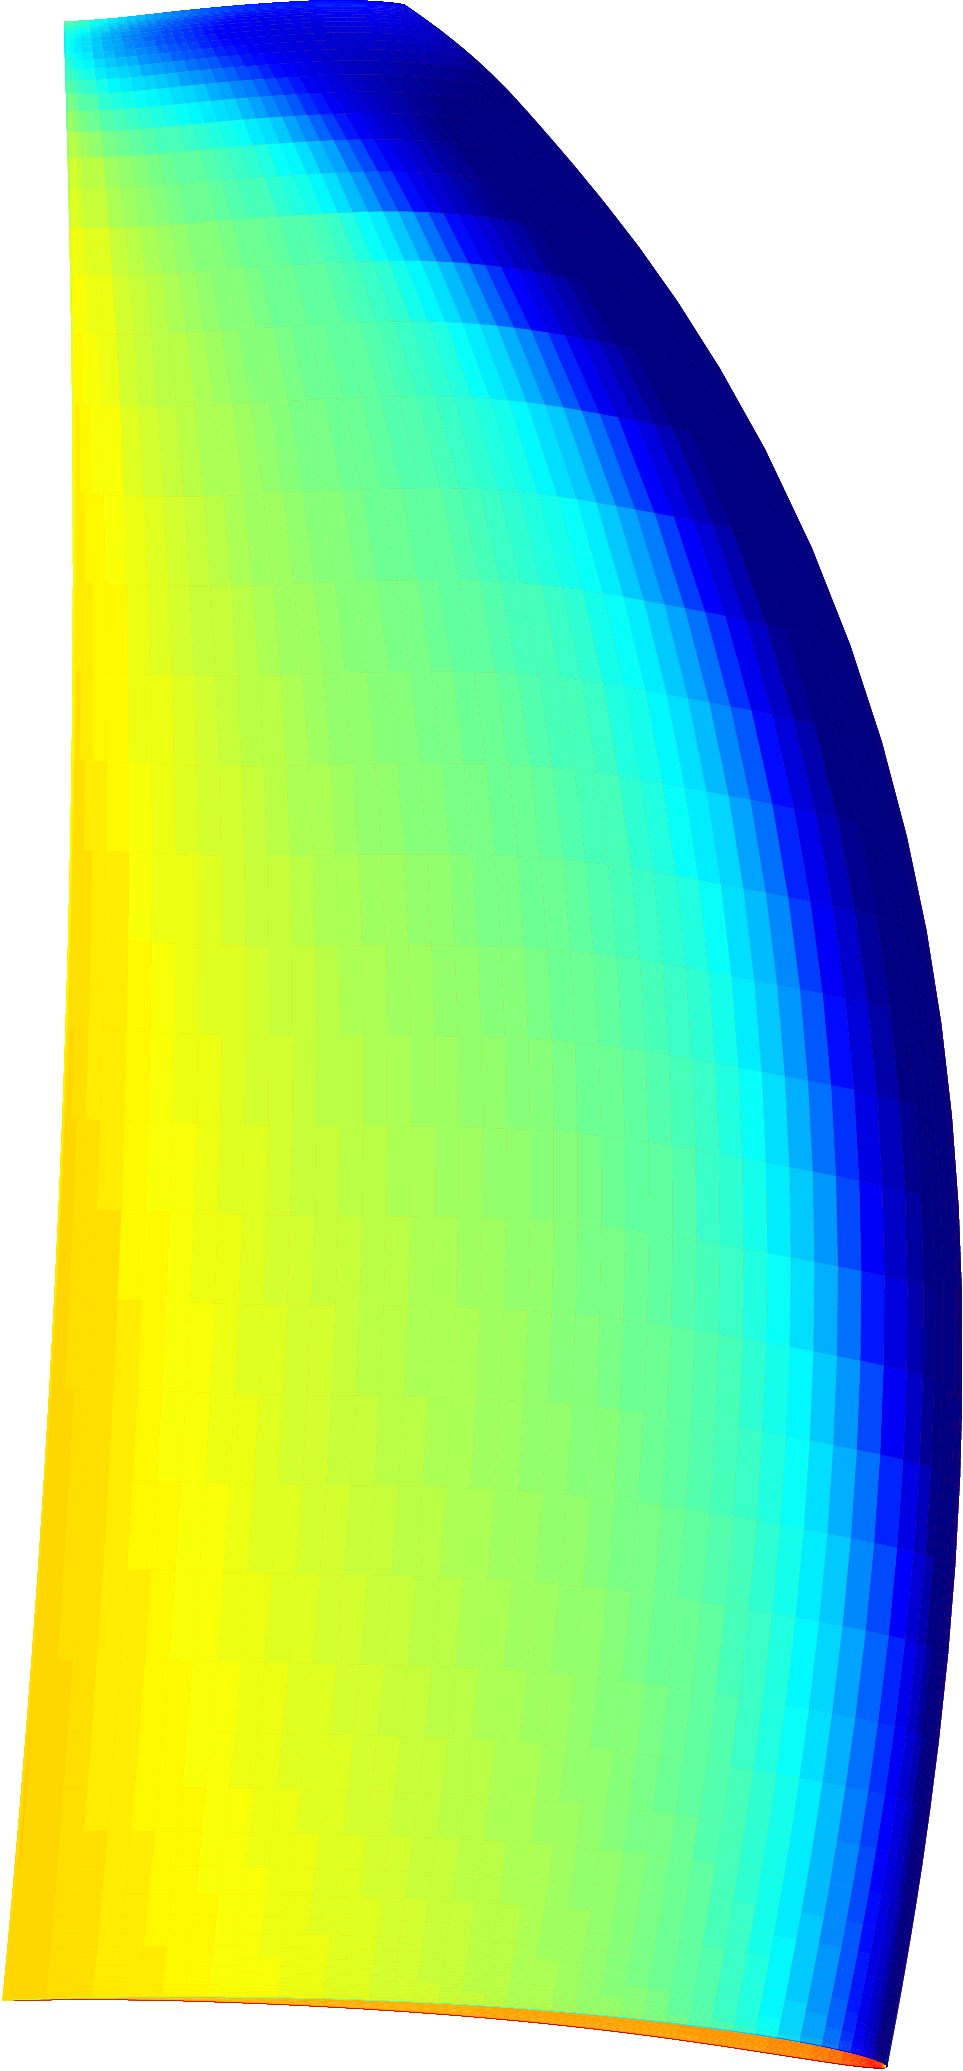
\includegraphics[width=0.10\textwidth]{DREAM_LS_TSM_N4_roe2_sa_blade_response_rear_mean_SS.png}
   & 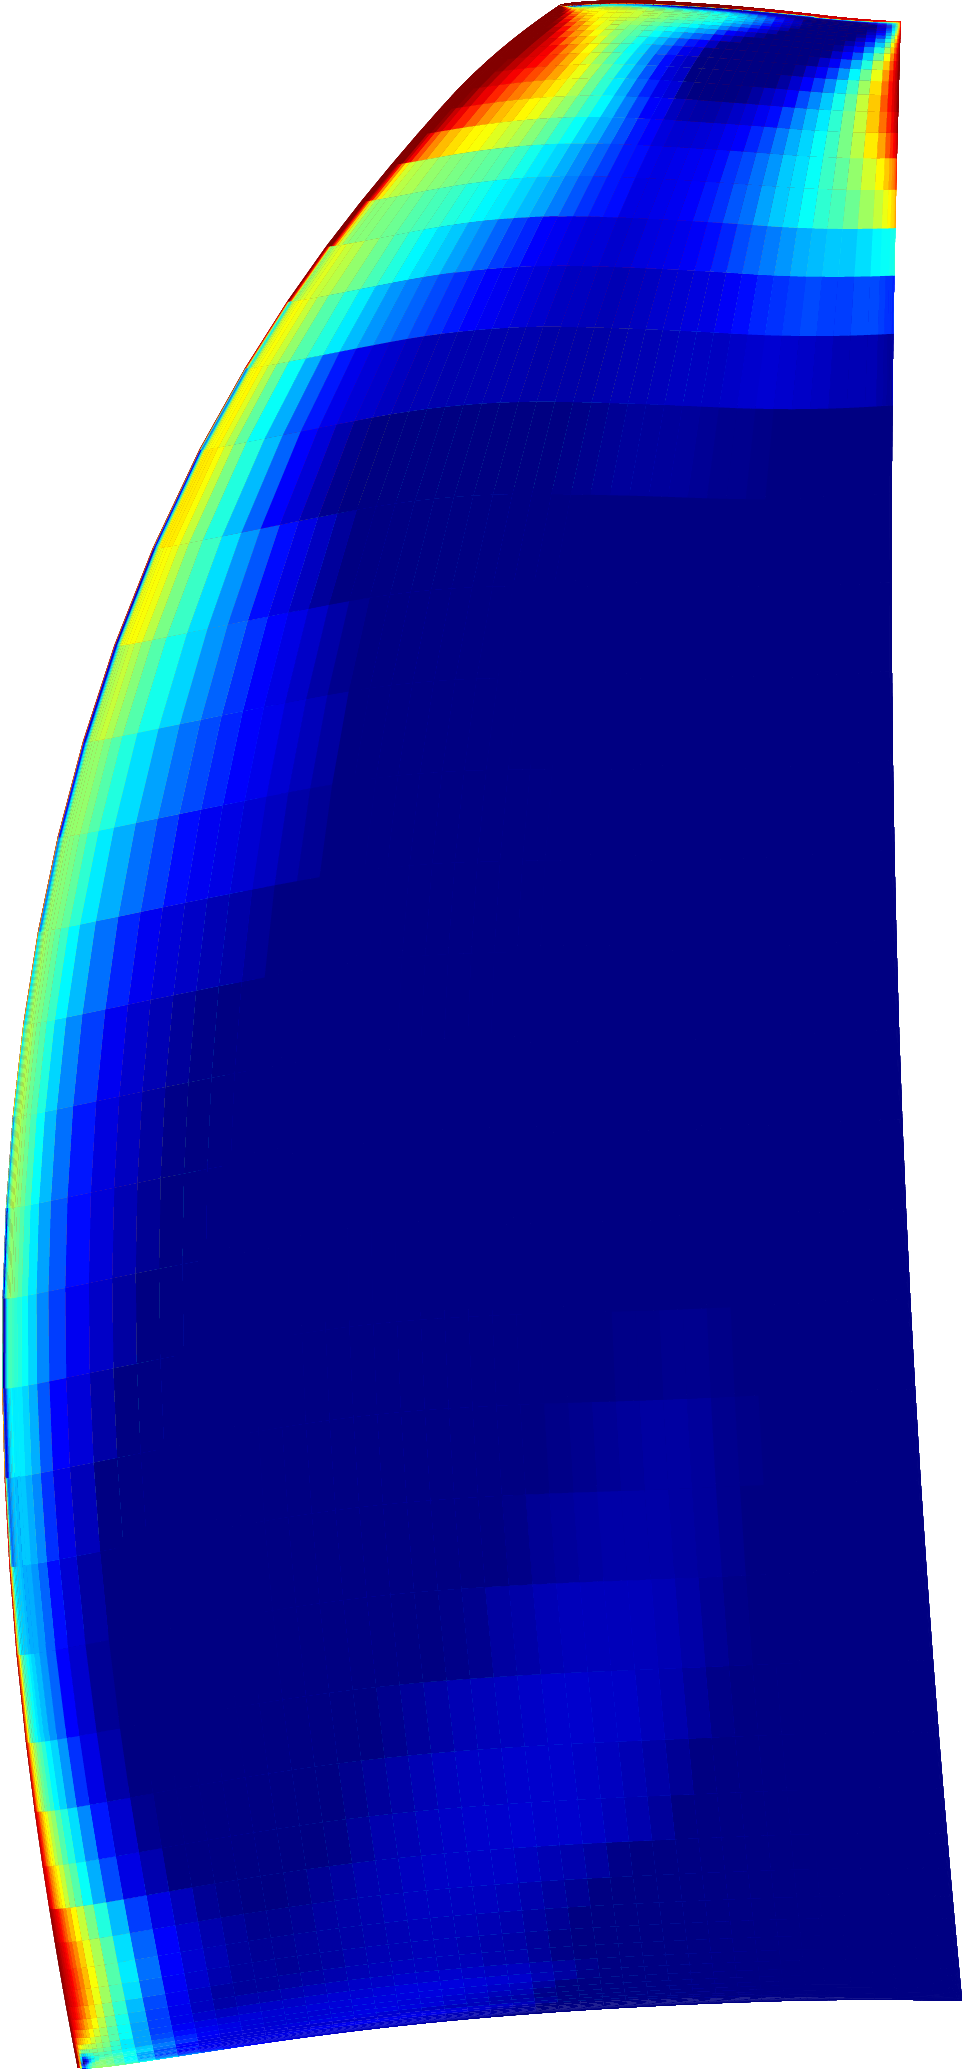
\includegraphics[width=0.10\textwidth]{DREAM_LS_TSM_N4_roe2_sa_blade_response_rear_H01_PS.png}
   & 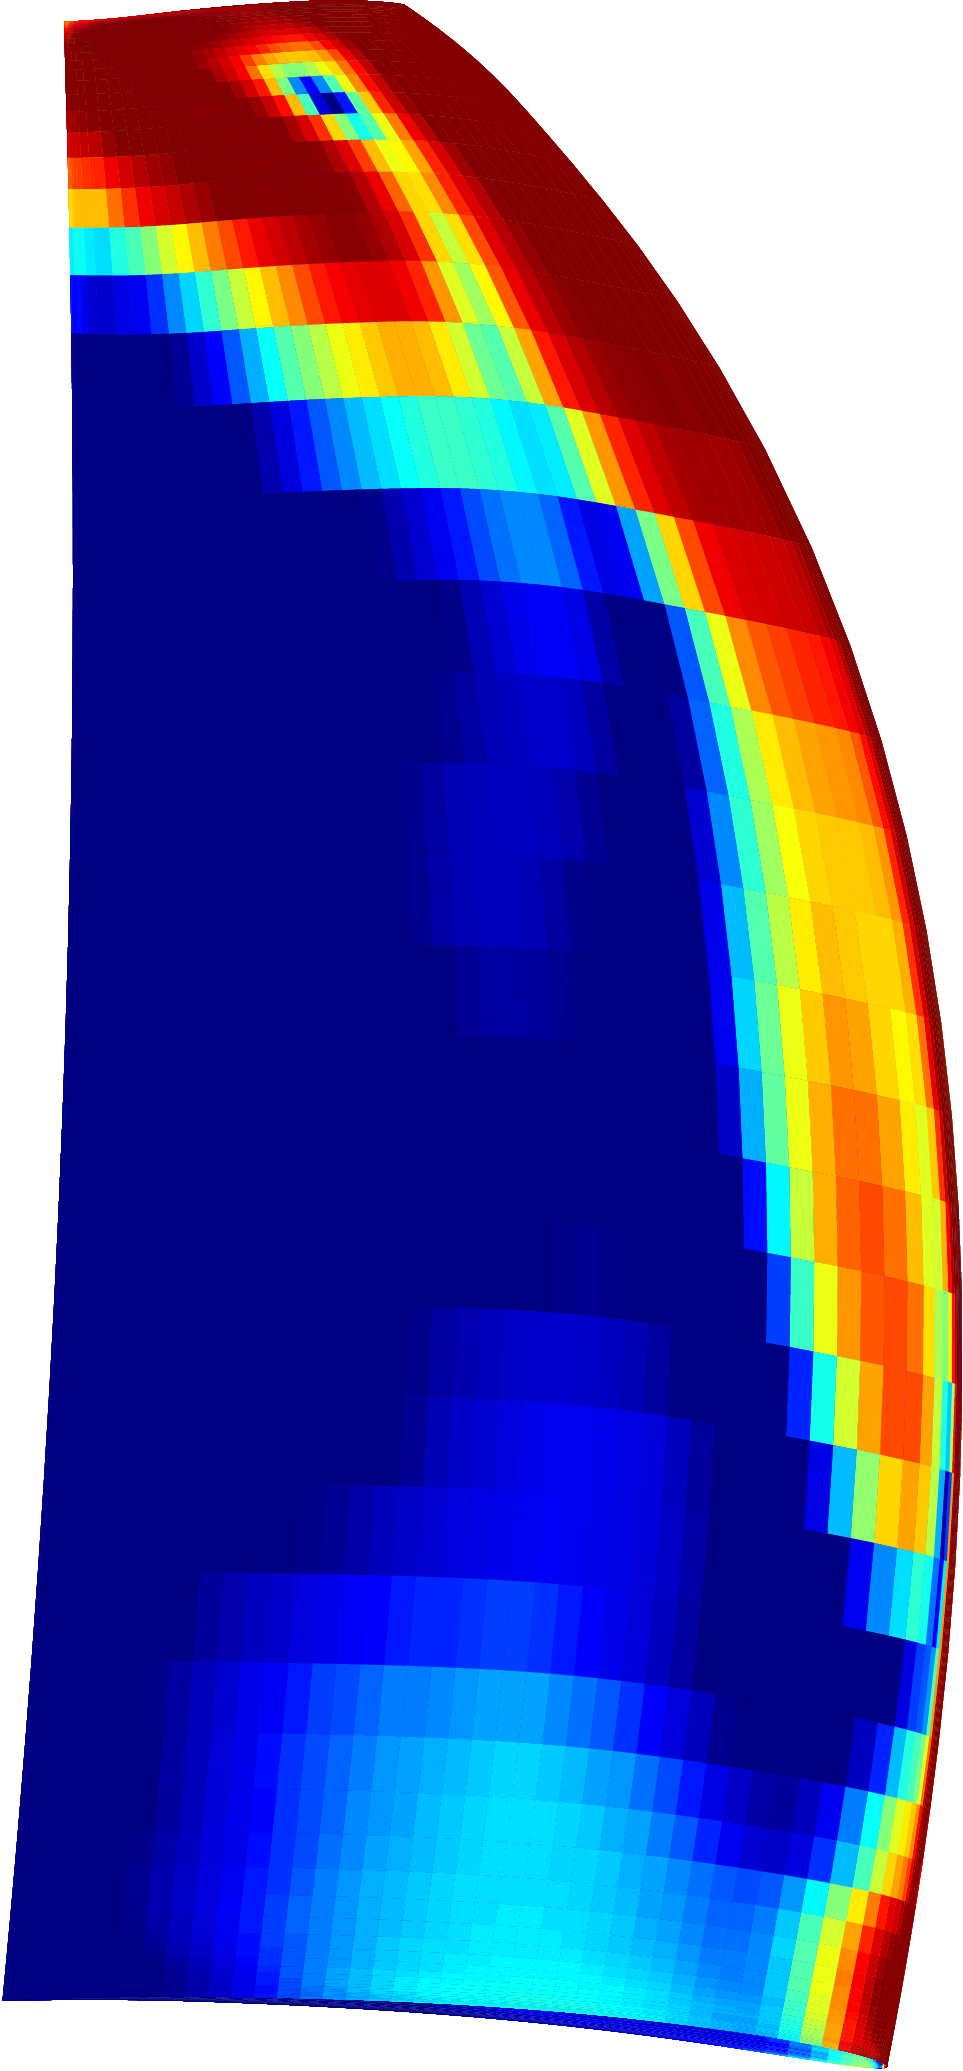
\includegraphics[width=0.10\textwidth]{DREAM_LS_TSM_N4_roe2_sa_blade_response_rear_H01_SS.png} \\
   \bottomrule
 \end{tabular}
 \caption{Low-speed isolated configuration: analysis of the number of harmonics
  required to capture the harmonic response of the rear rotor blades.}
 \label{fig:dream_ls_hb_blade_response_conv}
\end{figure}

\subsection{Residual convergence} 
\label{sub:dream_ls_hb_convergence_res}

\begin{figure}[htp]
  \centering
  \includegraphics*[width=0.5\textwidth]{DREAM_LS_TSM_COMPARISON_RESIDUALS_PPT.pdf}
  \caption{Low-speed isolated configuration: convergence of the residuals
  for the harmonic balance computations.}
  \label{fig:DREAM_LS_TSM_COMPARISON_RESIDUALS_PPT}
\end{figure}

\subsection{Integrated results: similarity coefficients}
\label{sub:dream_ls_hb_sim_coeff}

\subsection{One-dimensional results: radial profiles}
\label{sub:dream_ls_hb_radial_profiles}

\subsection{Two-dimensional results: radial and axial cuts}
\label{sub:dream_ls_hb_axial_radial_cuts}
